\section{Final BNF}\label{sec:final-bnf}

\begin{verbatim}
<stmtlist> ::=  <stmt> 
              | <stmt> <stmtlist>
<stmt> ::=  <expr> 
          | <vardecl>
          | <assertion>
          | <typealias>

<vardecl> ::= "let" <identifier> "=" <expr>
            | "let" <identifier> ":" <type> "=" <expr>
            | "let rec" <identifier> "=" <lambda>
            | "let async" <identifier> "=" <lambda>

<assertion> ::= "assert" <expr> | "assert" <expr> <string>

<typealias> ::= "type" <identifier> "=" <type>

<expr> ::=  <term> 
          | <term> "+" <expr> 
          | <term> "-" <expr>
          | <term> "==" <expr>
          | <term> "!=" <expr>
          | <term> "<" <expr>
          | <term> ">" <expr>
          | <term> "<=" <expr>
          | <term> ">=" <expr>
          | <term> "&&" <expr>
          | <term> "||" <expr>
            
<term> ::=  <factor> 
          | <factor> "*" <term> 
          | <factor> "/" <term> 
          | <factor> "%" <term> 
<factor> ::=  <literal> 
            | "(" <expr> ")" 
            | <factor> "^" <factor>
            | <factor> <userop> <factor>
            | <unaryop> <factor>
            | <factor> "(" <exprlist> ")"
            | <factor> "." <identifier>
            | <factor> "[" <expr> "]"
            | <factor> "[" <expr> ":" <expr> "]"
            | <factor> "[" <expr> ":" "]"
            | <factor> "[" ":" <expr> "]"
            | <factor> "." <identifier>
            | <range>
            | <if>
            | "${" <expr> "}"
            | "{" <stmtlist> "}"
            | <cast>

<cast> ::= <expr> ":" <type>

<unaryop> ::= "-" | "!" | "+" | <userop>
<userop> ::= <opchar> | <opchar> <userop>
<opchar> ::=  "!" | "@" | "#" | "$" | "%" | "^" | "&" 
            | "*" | "-" | "+" | "=" | "<" | ">" | "?" | ":" | "|" | "~"

<range> ::= "[" <expr> ".." <expr> "]"

<if> ::=  "if" <expr> "then" <expr> "else" <expr>
        | "if" <expr> "then" <expr>
        | <expr> "if" <expr> "else" <expr>

<literal> ::= <number> | <identifier> | <bool> | <list> | <lambda> | <string> | "()" | <tuple> | <record>
<string> ::= '"' <charlist> '"' | '""'
<charlist> ::= <char> | <char> <charlist>
<list> ::= "[" <exprlist> "]"
<tuple> ::= "(" <exprlist> ")"
<record> ::= "{" <recordlist> "}"
<recordlist> ::=  <identifier> "=" <expr> 
                | <identifier> "=" <expr> "," <recordlist>
                | <identifer> ":" <type> "=" <expr> 
                | <identifier> ":" <type> "=" <expr> "," <recordlist>

<lambda> ::=  "(" <typedexprlist> ")" "->" <expr>
            | "(" <typedexprlist> ")" ":" <type> "->" <expr>
            | "(" <typedexprlist> ")" "{" <stmtlist> "}"
            | "(" <typedexprlist> ")" ":" <type> "{" <stmtlist> "}"

<bool> ::= "true" | "false"

<number> ::= <int> | <float> | <rational>
<int> ::= <digit> | <digit> <int>
<float> ::= <int> "." <int>
<rational> ::= <int> "/" <int>
<complex> ::= <float> "+" <float> "i" | <float> "-" <float> "i" | <float> "i"
<digit> ::= "0" | "1" | "2" | "3" | "4" | "5" | "6" | "7" | "8" | "9"

<identifier> ::= <letter> | <letter> <identifier>
<letter> ::=  "a" | "b" | "c" | "d" | "e" | "f" | "g" | "h" | "i" | "j" | "k" | "l" | "m" 
            | "n" | "o" | "p" | "q" | "r" | "s" | "t" | "u" | "v" | "w" | "x" | "y" | "z"

<exprlist> ::= <expr> | <expr> "," <exprlist>
<typedexprlist> ::=  <expr> ":" <type> 
                   | <expr> ":" <type> "," <typedexprlist>
                   | <expr> "," <typedexprlist>

<type> ::=  "int" | "float" | "bool" 
          | "(" <typelist> ")" "->" <type> 
          | "[" <type> "]" | "(" <typelist> ")"
          | "{" <recordtypelist> "}"
          | <identifier>

<recordtypelist> ::= <identifier> ":" <type> | <identifier> ":" <type> "," <recordtypelist>

<typelist> ::= <type> | <type> "," <typelist>
\end{verbatim}

This BNF is represented in the F\# codebase as an AST, represented by the following type:

\begin{minted}{fsharp}
/// <summary>
/// The AST of the language.
/// </summary>
type Expr =
    | ELiteral of Literal * Type
    | EIdentifier of Token * Type option
    | EGrouping of Expr * Type option

    | EIf of Expr * Expr * Expr * Type option
    | ETernary of Expr * Expr * Expr * Type option

    | EList of Expr list * Type option
    | ETuple of Expr list * Type option

    | ECall of Expr * Expr list * Type option

    /// <summary>
    /// Indexing operation on a list or tensor.
    /// Expr (list or tensor), (index), type
    /// Allows for indexing in the form l[1]
    /// </summary>
    | EIndex of Expr * Expr * Type option

    /// <summary>
    /// Indexing with a range operation on a list or tensor.
    /// Expr (list or tensor), start, end, type
    /// Allows for indexing in the form l[..1] or l[1..2] or l[1..]
    /// </summary>
    | EIndexRange of Expr * Expr * Expr * Type option

    /// <summary>
    /// A lambda expression with a list of arguments, a body, a return type, a pure flag, and a type.
    /// </summary>
    | ELambda of (Token * Type option) list * Expr * Type option * bool * Type option * bool // bool is pure flag
    | EBlock of Stmt list * bool * Type option // bool is whether block is part of a function
    | ERange of Expr * Expr * Type option

    | ERecordSelect of Expr * Token * Type option

    /// <summary>
    /// Records represented recursively as a row type.
    /// </summary>
    | ERecordExtend of (Token * Expr * Type option) * Expr * Type option
    | ERecordRestrict of Expr * Token * Type option
    | ERecordEmpty of Type

    /// <summary>
    /// Unevaluated code block.
    /// </summary>
    | ECodeBlock of Expr

    /// <summary>
    /// A tail call (for tail recursion).
    /// </summary>
    | ETail of Expr * Type option

/// <summary>
/// A statement in the language (something that does not return a value).
/// </summary>
and Stmt =
    | SExpression of Expr * Type option
    | SVariableDeclaration of Token * Expr * Type option
    | SAssertStatement of Expr * Expr option * Type option
    | STypeDeclaration of Token * Type * Type option
    | SRecFunc of Token * (Token * Type option) list * Expr * Type option
    | SAsync of Token * (Token * Type option) list * Expr * Type option
    | SImport of Token option * string * bool * Type option // maybe binding name, module name (path), isstd, type
\end{minted}

\section{Final GUI}\label{sec:final-gui}

The final GUI is shown in subsections~\ref{subsec:code-editor},~\ref{subsec:notebook-view} and~\ref{subsec:plot-view}.
It has 3 types of windows: the code editor, the notebook view and the plot view.
It has support for loading in a file, buttons for running or transpiling the code, and an interactive repl.
The notebook view supports importing or exporting from a proprietary file format, running code blocks and exporting 
to a PDF\@.

\begin{figure}[H]
    \centering
    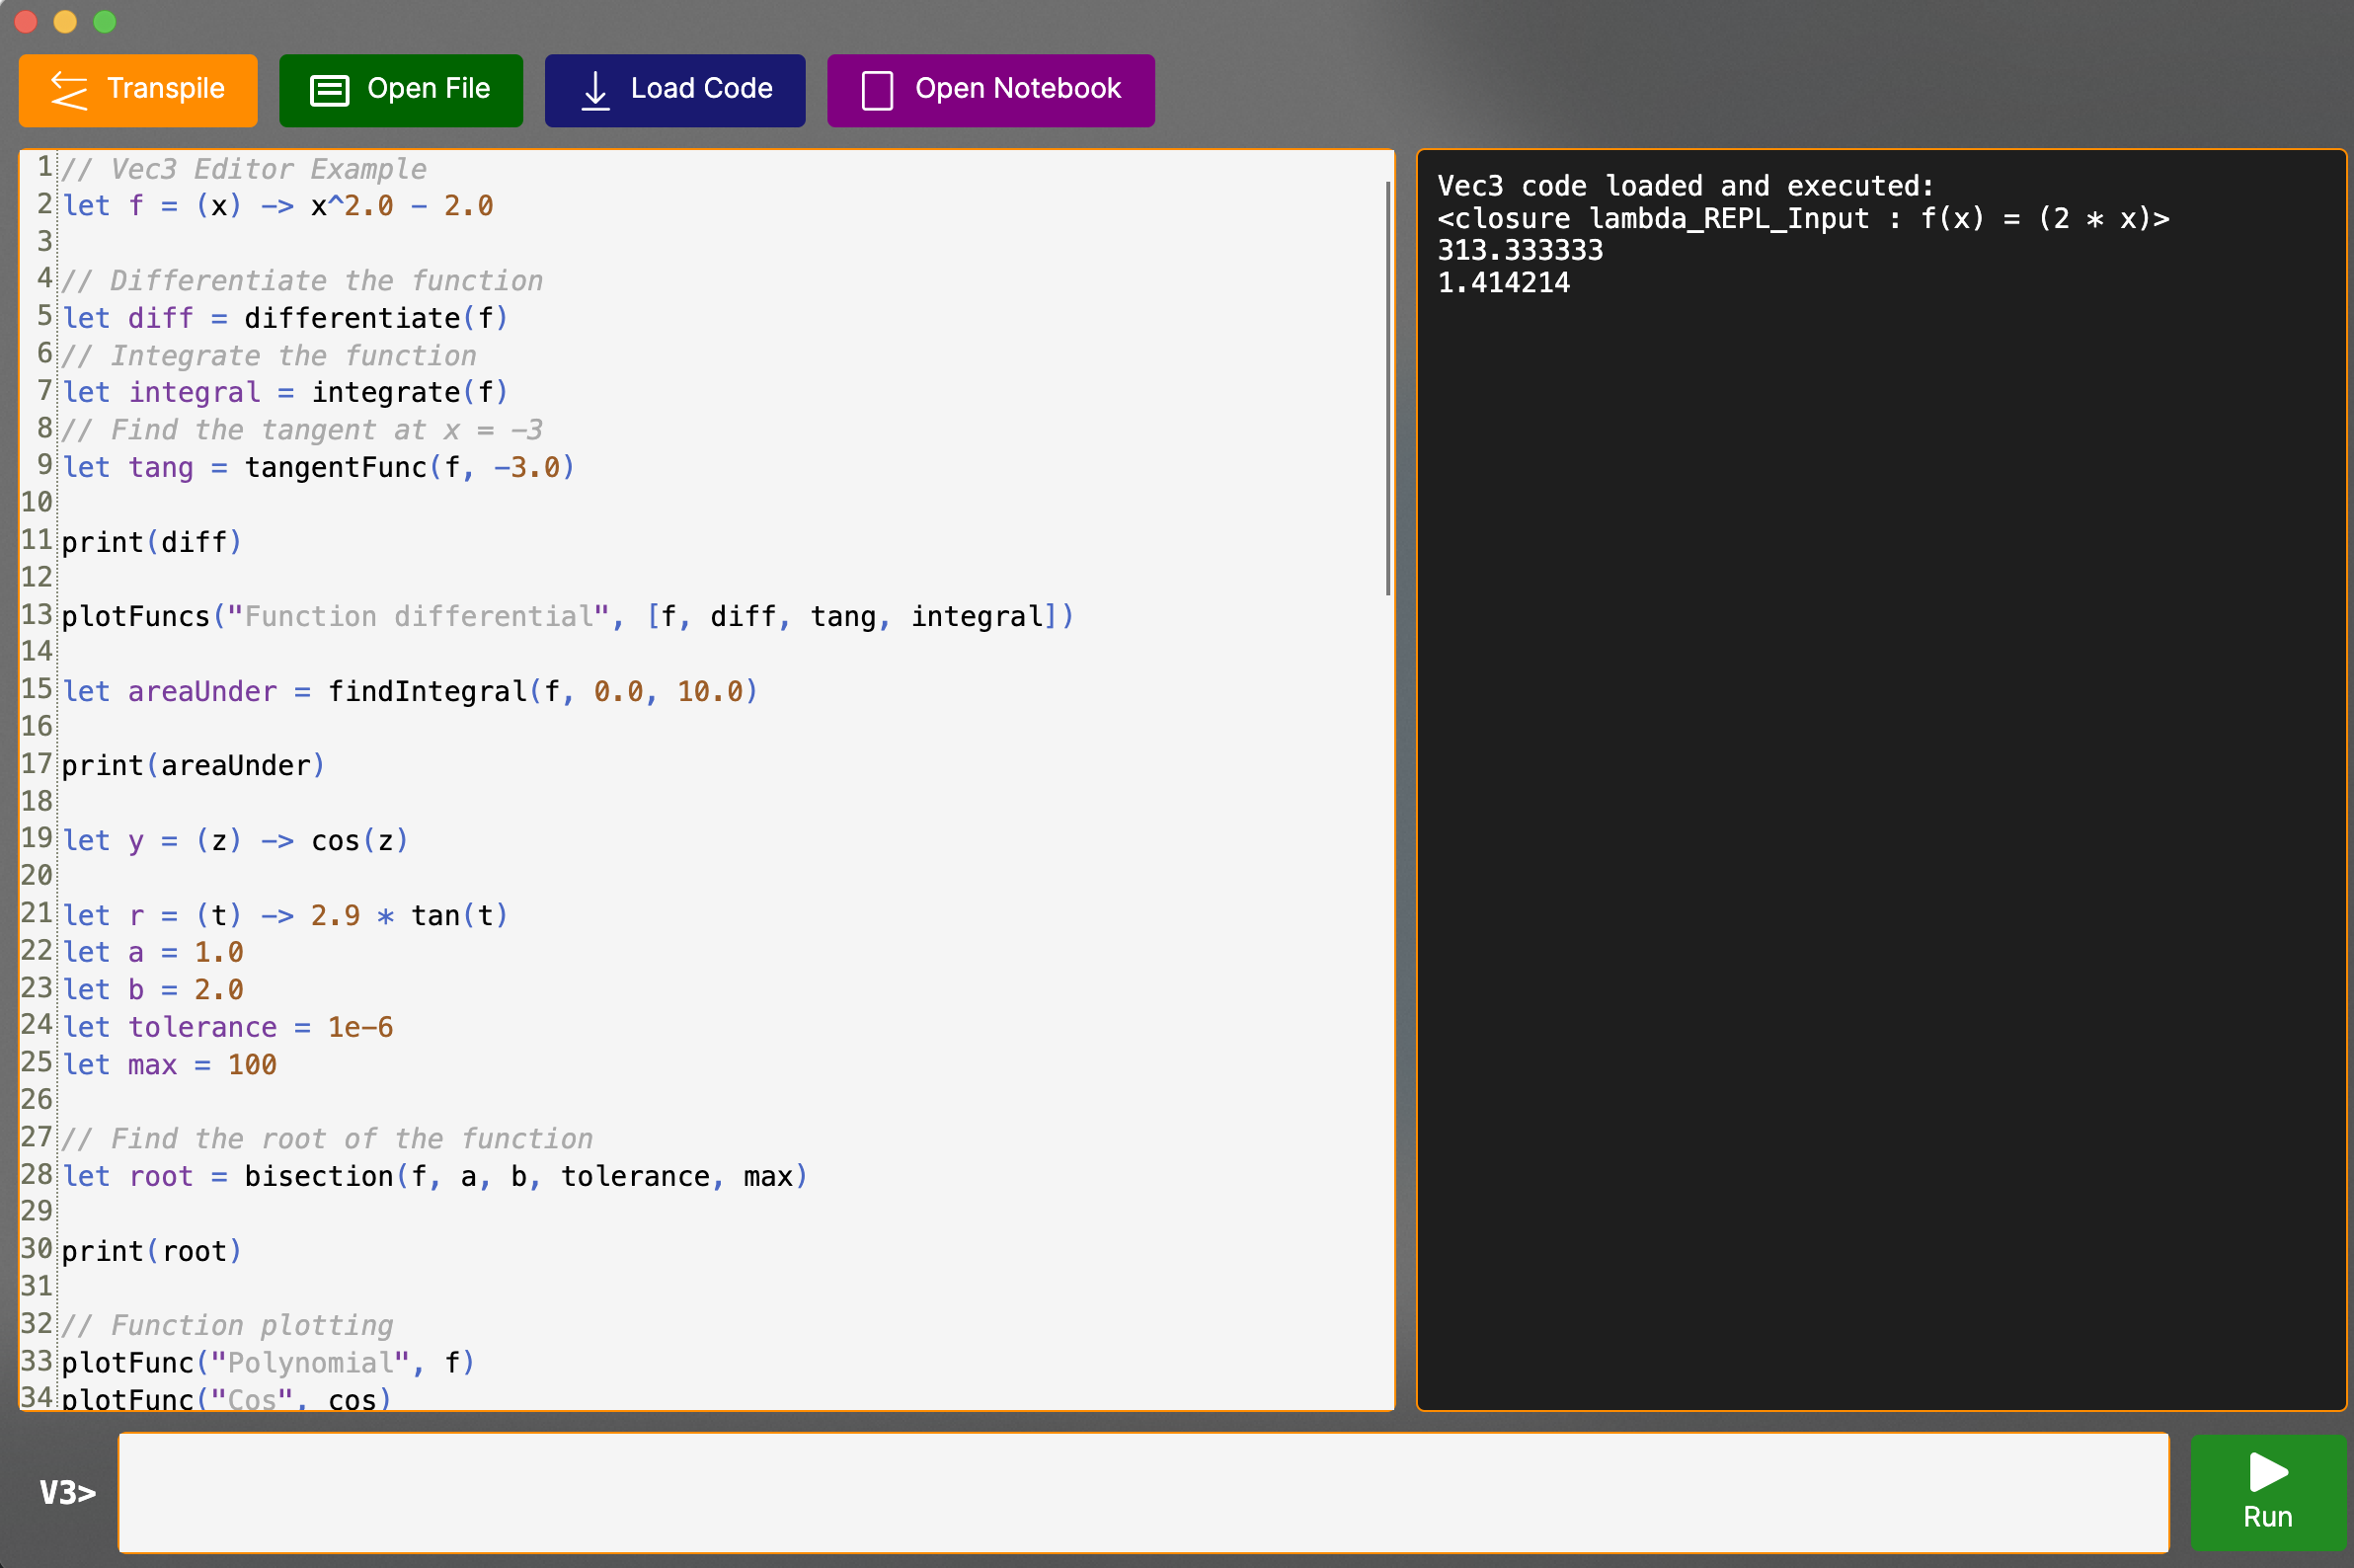
\includegraphics[width=0.8\textwidth]{assets/finalCodeEditor}
    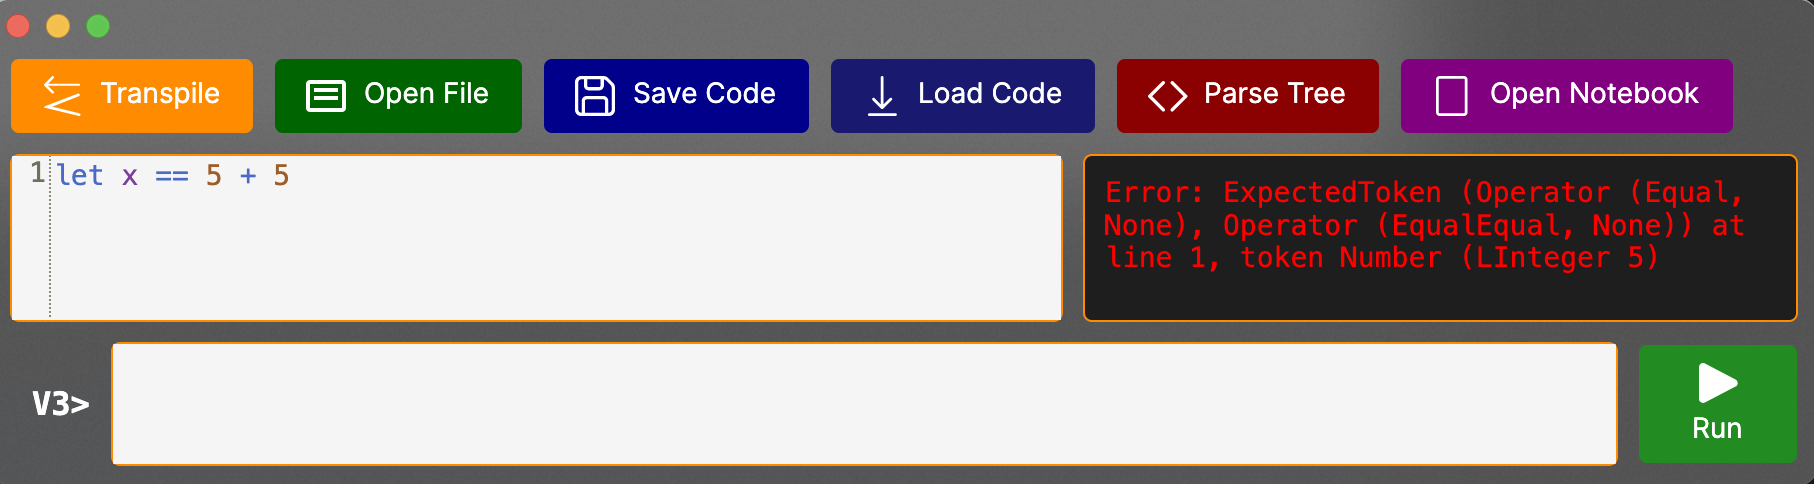
\includegraphics[width=0.8\textwidth]{assets/finalGuiParserError}
    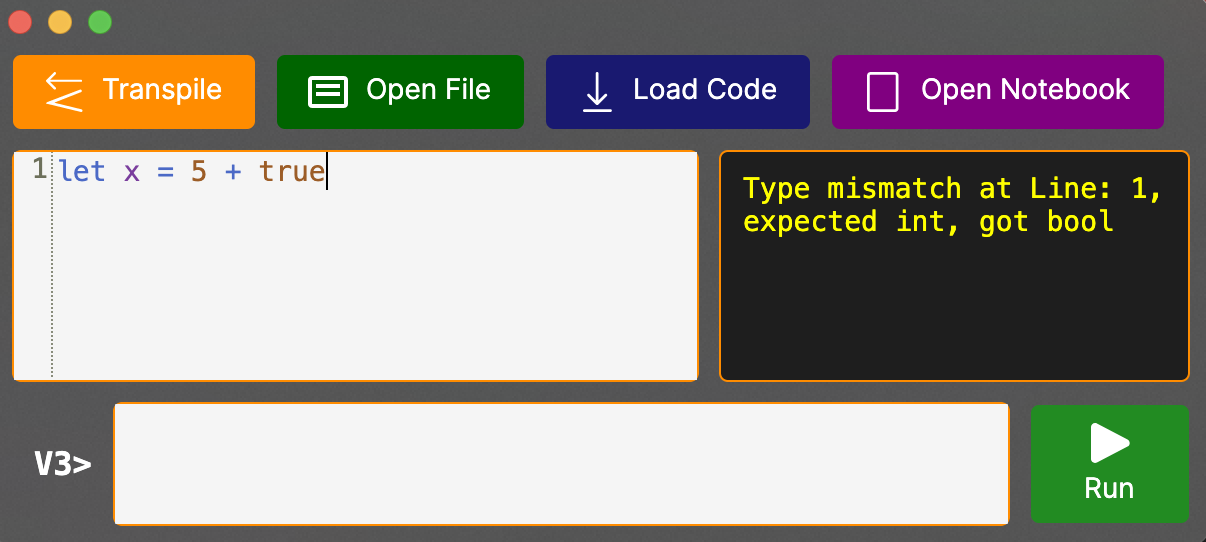
\includegraphics[width=0.8\textwidth]{assets/finalGuiTypeError}
    
\includegraphics[width=0.8\textwidth]{assets/finalREPL}
    \caption{Final GUI}\label{fig:final-gui}
\end{figure}

\subsection{Code Editor}\label{subsec:code-editor}

The code editor is where the user writes their code, and is the main window of the GUI\@.
It has syntax highlighting, live error checking and a REPL\@.

Images are given in figure~\ref{fig:final-gui} of the code editor with output, live parser errors and live type errors.

\subsection{Notebook View}\label{subsec:notebook-view}

The notebook view is where the user can write code in a more interactive way, similar to Jupyter notebooks\citep{Jupyter}.
It has support for importing or exporting from a proprietary file format, running code blocks and exporting to a PDF\@.
An image is shown in figure~\ref{fig:notebook-view}.
As shown, variable assignment persists between code blocks, the result of the code block is displayed below the code
and plotting functions are supported.

\begin{figure}[H]
    \centering 
    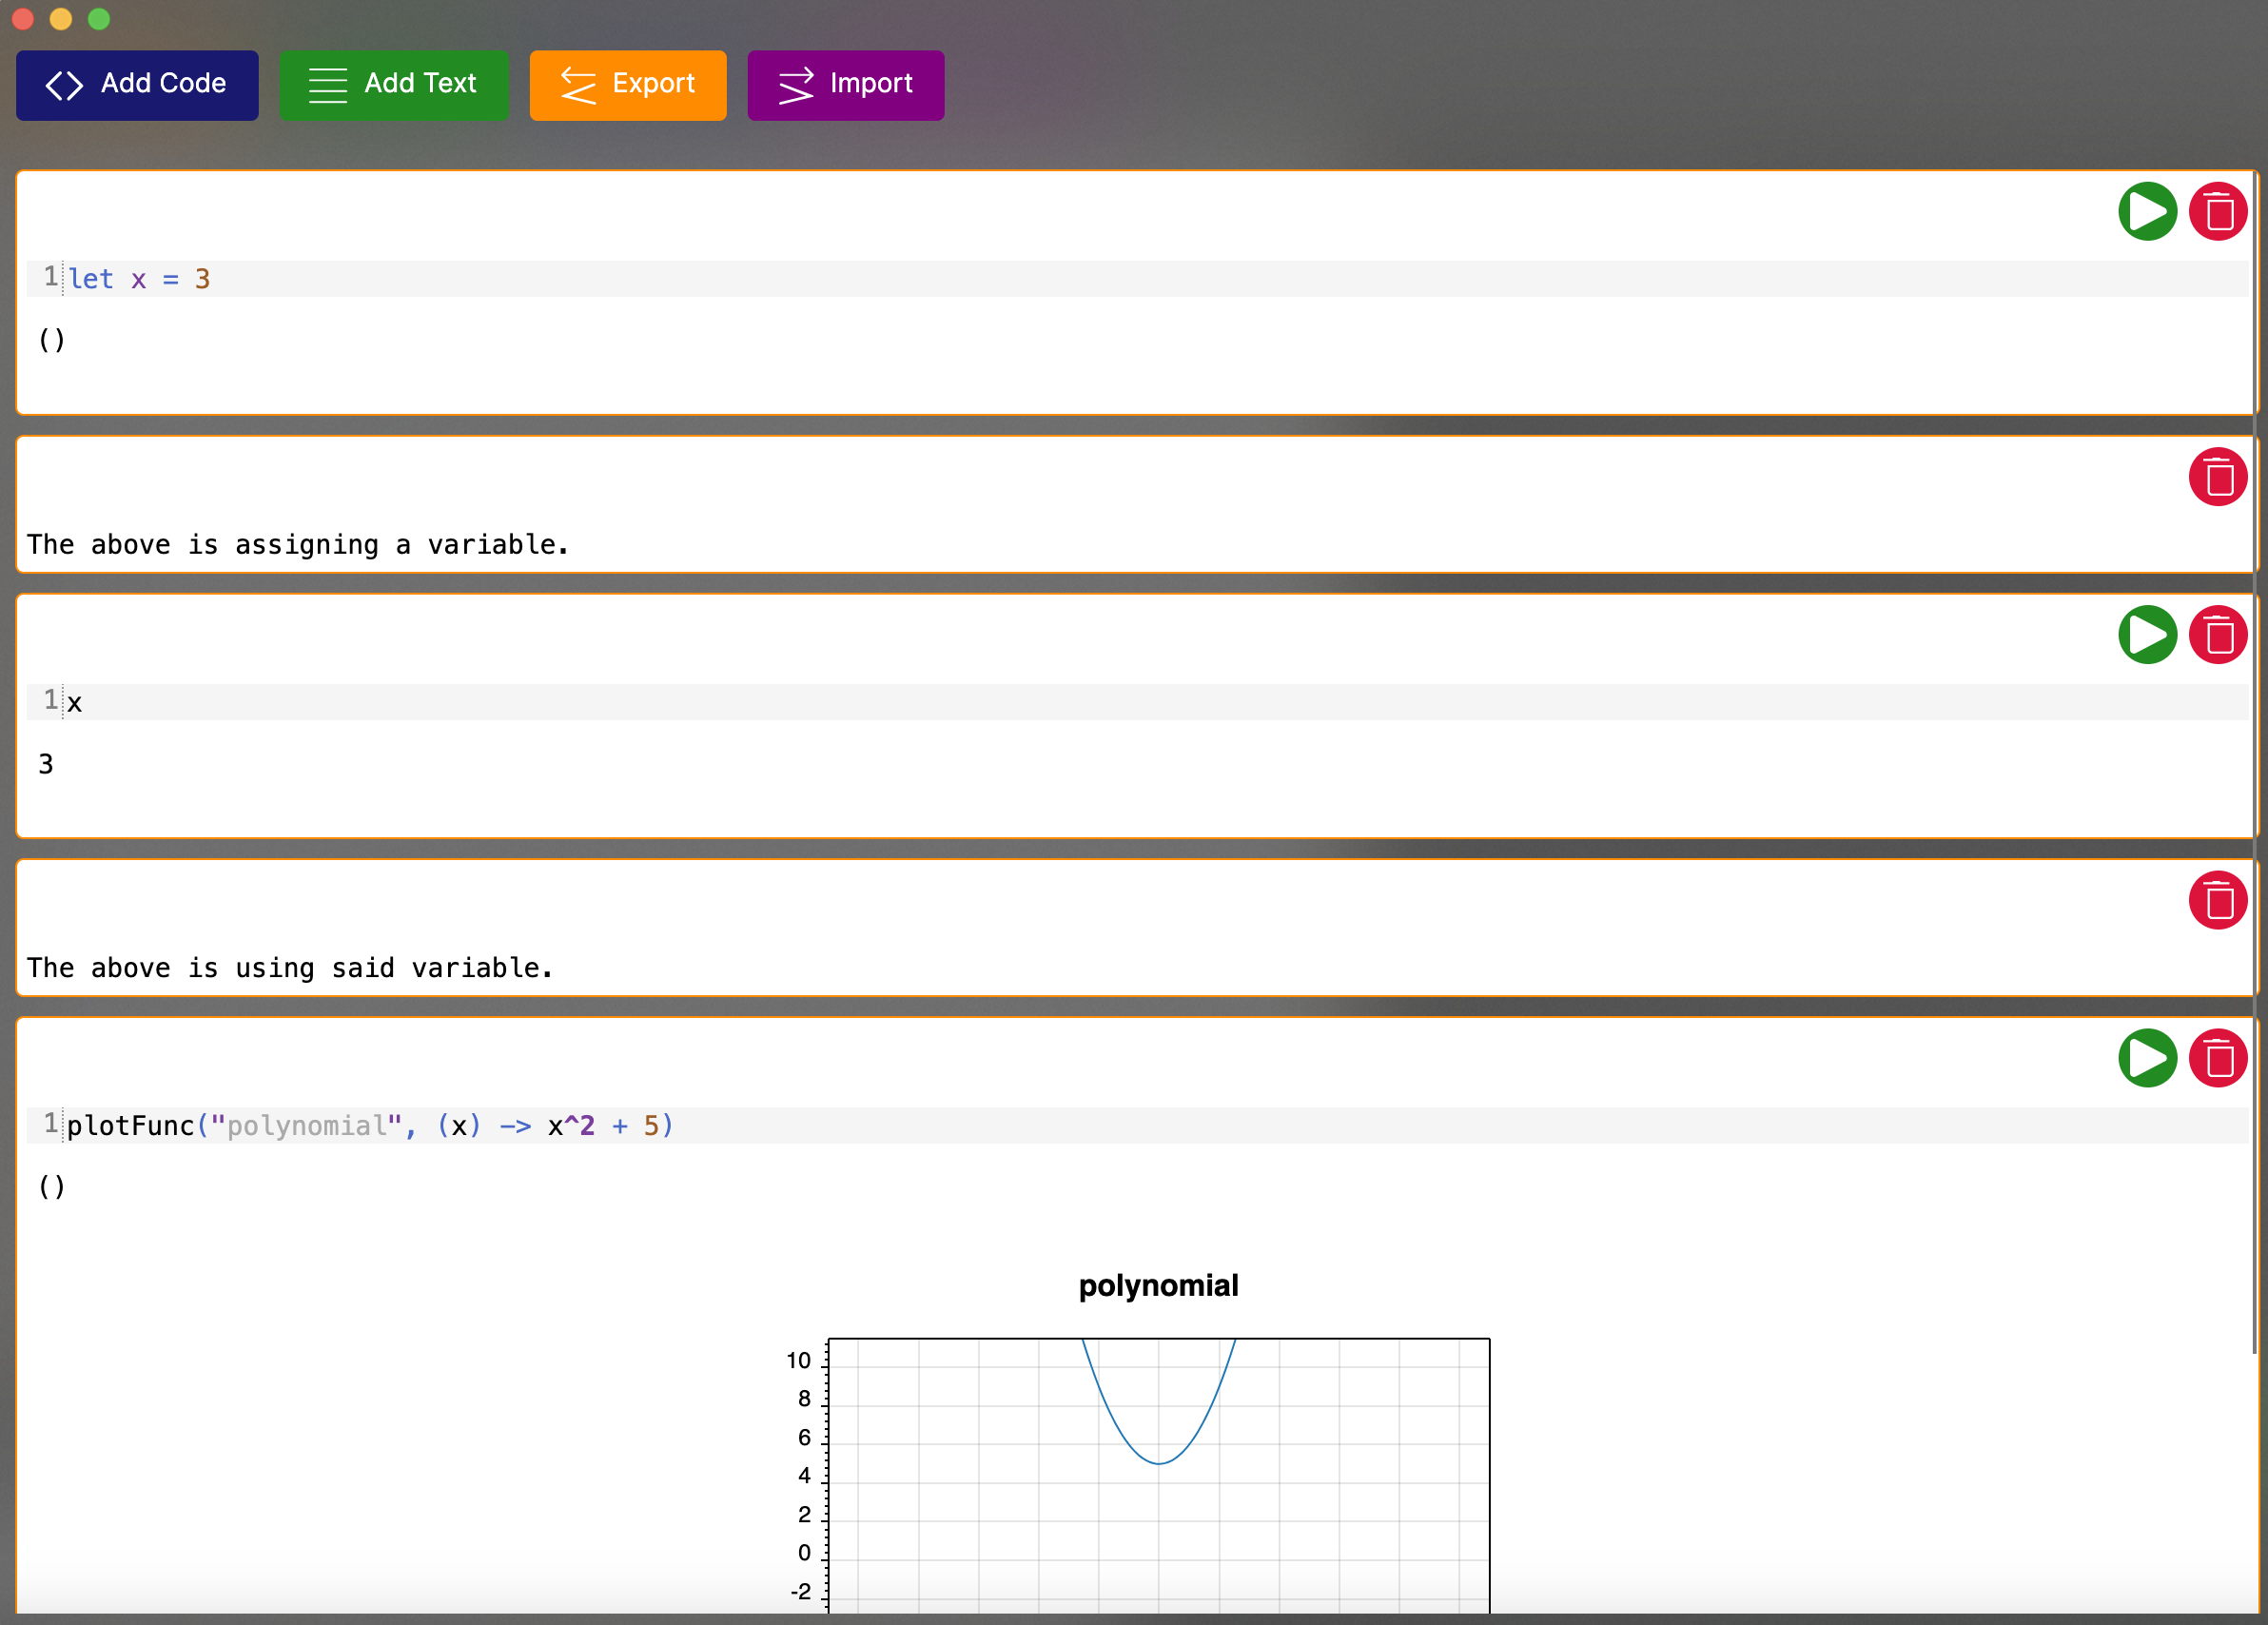
\includegraphics[width=0.8\textwidth]{assets/finalNotebook}
    \caption{Notebook view}\label{fig:notebook-view}
\end{figure}

An example PDF export from the given image is shown in figure~\ref{fig:pdf-export}.

\begin{figure}[H]
    \centering
    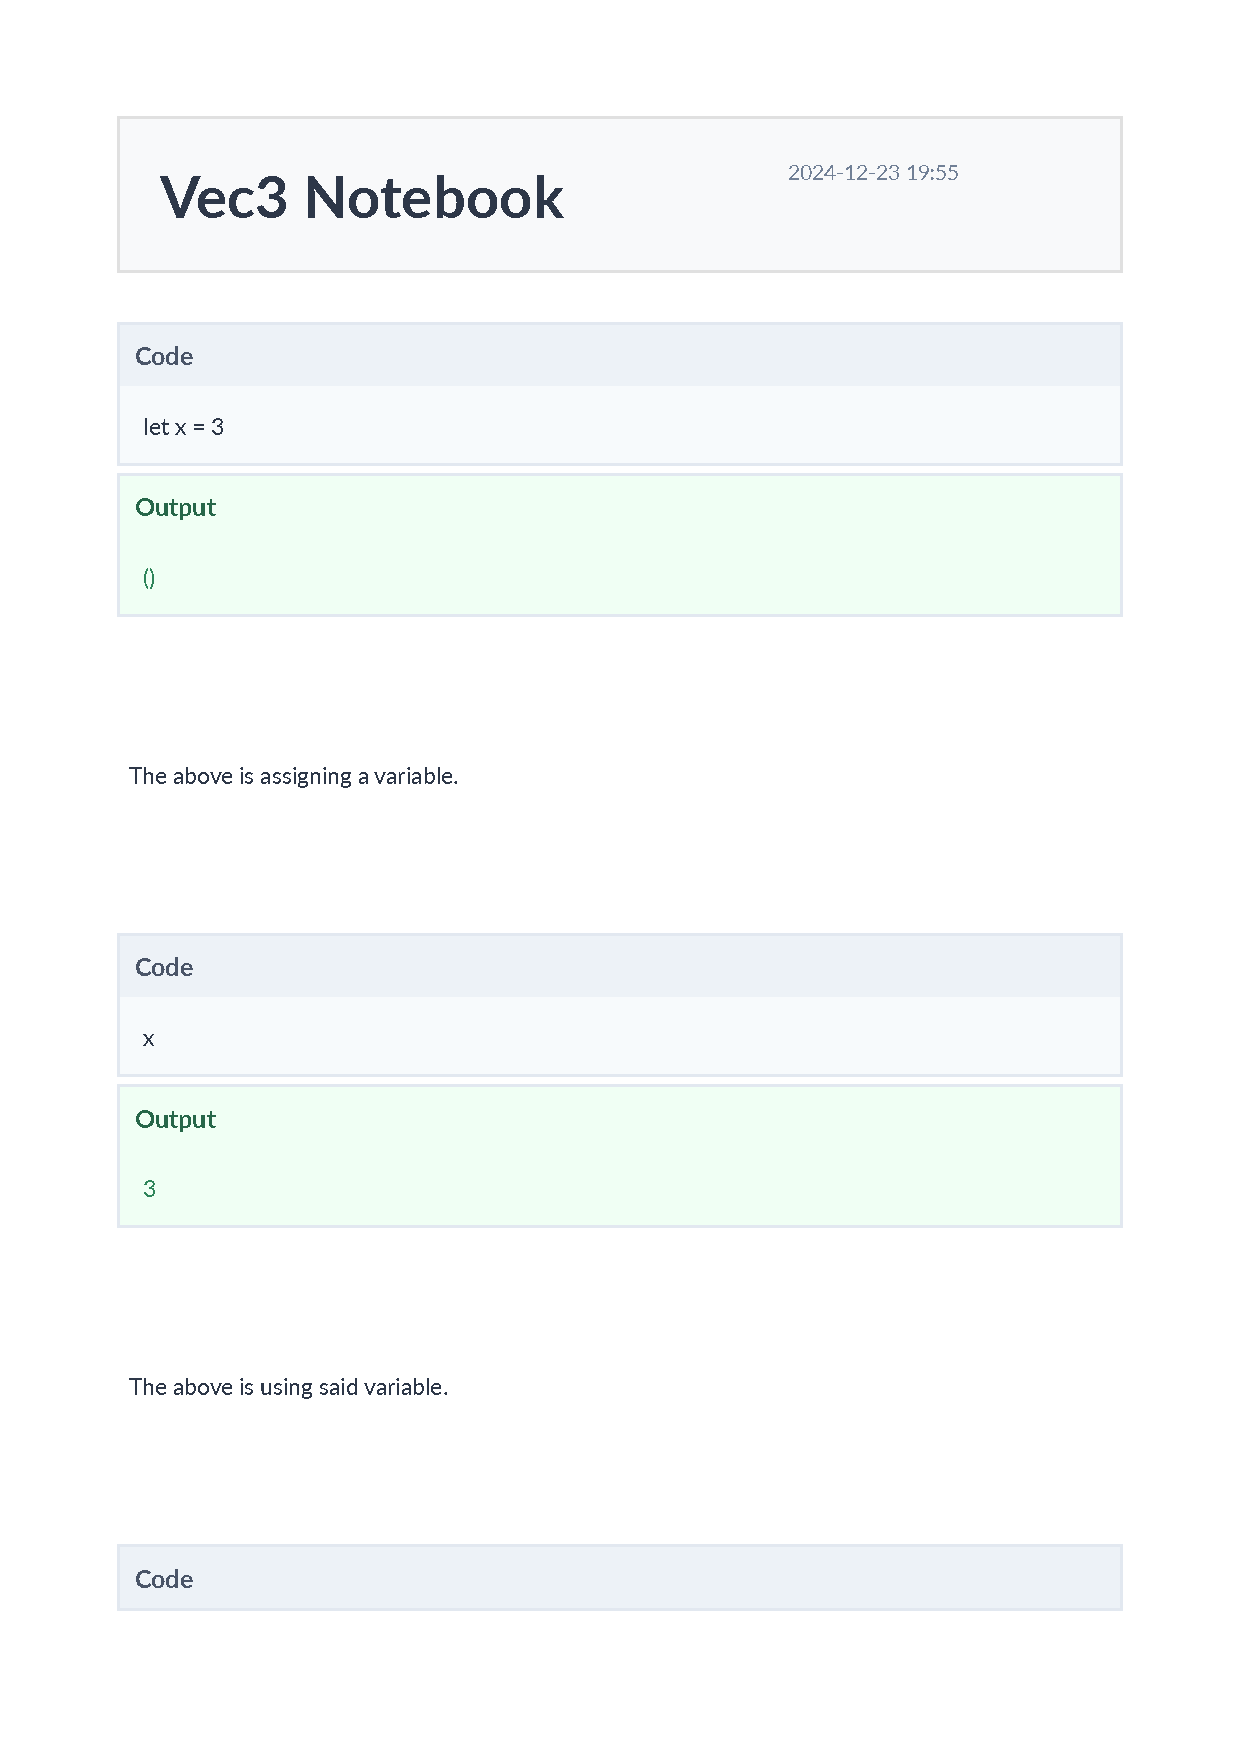
\includegraphics[page=1,width=0.8\textwidth]{assets/plotPDF}
    \includegraphics[page=2,width=0.8\textwidth]{assets/plotPDF}
    \caption{PDF export}\label{fig:pdf-export}
\end{figure}

\subsection{Plot View}\label{subsec:plot-view}

The plot view is where the user can view plots generated by the code.
It has support for zooming in and out, moving around and adjusting the axes, as well as interactive input for
plotting functions.
Images and further details are given in section~\ref{sec:plotting}.

\subsection{REPL}\label{subsec:repl}

The main view also includes a REPL input at hte bottom, allowing the user to interact with the program in a more
interactive way.
After running the code, the user can type expressions in the REPL and have them evaluated, with the result being
displayed on the right.
Note that the results don't have to be explicitly printed, as the REPL will display the result of the last expression
evaluated.
An image is shown in figure~\ref{fig:final-gui}.

\subsection{Syntax Window}\label{subsec:syntax-window}

A window containing examples of the syntax of the language is also included, allowing the user to quickly see how to
write certain expressions or functions.
This is accessed by typing \textit{help()} in the REPL\@.

\section{Notable Features}\label{sec:notable-features}

Alongside standard arithmetic operations, variable assignment, function definitions, and plotting the language also 
supports the following interesting features:

\paragraph{User defined operators} The user can define their own operators, both unary and binary, with the 
following syntax:

\begin{minted}{fsharp}
// Define a binary operator
let (|+|) = (a: float, b: float) -> a + b

// Define a unary operator
let (|!|) = (a: bool) -> not a
\end{minted}

This is a powerful feature allowing for the language to be extended in a way that is meaningful to the user.

\paragraph{Static type inference} The language uses Hindley-Milner type inference to infer the types of
expressions while giving the user the option of specifying types explicitly, improving the correctness of the
code and reducing the cognitive load on the user.

\begin{minted}{fsharp}
let f = (x: float) -> x + 1.0
let f: (float) -> float = (x) -> x + 1.0
let f = (x: float) : float -> x + 1.0
\end{minted}

\paragraph{Compound data types} The language supports compound data types such as lists, tuples and records,
allowing for more complex data structures to be represented.

\begin{minted}{fsharp}
let l = [1, 2, 3]
let l1 = l[0]

let t = (1, true, "this is a tuple")

let r = { x = 1, y = 2 }
let r1 = r.x
\end{minted}

\paragraph{Imports} The language supports importing other files, allowing for code to be split across multiple
files, improving code organisation and reusability.
As well as this, a small standard library has been written that can be imported as desired.

\begin{minted}{fsharp}
import "file.vec3"
import "list"

let f = (x) -> func(x) // func defined in file.vec3
let l = [1, 2, 3]
let l1 = head(l) // head defined in list
\end{minted}

\paragraph{Turing Completeness} The language is Turing complete, allowing for the implementation of any
algorithm that can be implemented in a Turing complete language.
As the language is immutable, this is done through recursion and higher order functions, with control flow
managed through if expressions.

\begin{minted}{fsharp}
let rec map = (list, f) -> if len(list) == 0 then [] else f (head(list)) :: map (tail(list), f)
\end{minted}

\paragraph{Calculus} The language has built-in functions for finding the integral function, derivative function
and tangent function at a given point of a function.
As such, a few useful math operations are built around these, such as finding the integral:

\begin{minted}{fsharp}
let findIntegral = (f, a, b) {
    let integral = integrate(f)
    integral(b) - integral(a)
}
\end{minted}

\paragraph{Vector and Matrix operations} The language represents vectors and matrices as lists of numeral types, with
operations such as addition, subtraction, multiplication and division defined for them, and functions such as \textit{transpose} and \textit{determinant} defined for matrices.

\begin{minted}{fsharp}
let v1 = [1.0, 2.0, 3.0]
let v2 = [4.0, 5.0, 6.0]
let v3 = v1 + v2

let m1 = [[1.0, 2.0], [3.0, 4.0]]
let trans = transpose(m1)
let det = determinant(m1)
let inv = inverse(m1)
\end{minted}


\paragraph{Async functions} The language supports asynchronous functions, allowing for non-blocking operations
to be performed.
This is useful is a long calculation is to be performed, as the function will run in the background until awaited.

\begin{minted}{fsharp}
let async longCalc = sum([1..1000000])

let result = await(longCalc)
\end{minted}

\paragraph{Range Expressions} The language supports range expressions, allowing for a list of numbers to be
generated easily.
In addition to this, list indexing also supports ranges, allowing for a sublist to be extracted from a list.

\begin{minted}{fsharp}
let l = [1..10]
let l1 = l[1..5] // Extracts the sublist [2, 3, 4, 5, 6]
let l2 = l[1..] // Extracts the sublist [2, 3, 4, 5, 6, 7, 8, 9]
let l3 = l[..5] // Extracts the sublist [1, 2, 3, 4, 5]
\end{minted}

\paragraph{Function Plotting} The language has built-in functions for plotting functions, allowing for easy
visualisation of functions.
This is done through the \textit{plotFunc} function, which takes in a function and plots it on a graph.

\section{Lexer}\label{sec:lexer}

Initial lexer design was based on a simple regular expression based lexer, but this was later replaced with a more
functional approach using pattern matching on the input string.
The reason for this change was that the regular expression based lexer was difficult to extend and maintain due to 
the lack of type safety.
For example if we had a more general regex called before a more specific one, the more general one would always match
first, even if the more specific one should have matched.

This was solved by using a more functional approach, where the type system of F\# would inform us if a case would 
never be matched due to the order of the cases or otherwise, preventing a class of easily overlooked errors during development.
The lexer is now implemented as a recursive pattern matching function that takes a string and returns a list of 
tokens, complete with their lexeme and position in the input string.

Lexer errors are also accumulated in a list of type \textit{LexerError}, which are displayed to the user in the GUI\@.

Something of note is that the lexer parses numbers itself, rather than passing them to the parser as strings.

Additionally, due to the permittance of user defined operators, the lexer makes special considerations when lexing 
special characters, as the distinction between a built-in operator (with precedence) and a user defined operator (
currently without taking precedence into account) is made during lexing.

Furthermore, both block comments (\textit{/* */}) and line comments (\textit{//}) are handled by the lexer by ignoring
the contents of the comment.
In future, it may be interesting represent comments as a token in the AST, allowing for systems such as documentation
generation or automatic formatting to be implemented.

\section{Parser}\label{sec:parser}

The parser is implemented using Pratt parsing\citep{pratt1973top}, which is a top-down operator precedence parsing 
method that allows for easy extension and modification of the grammar.
It works by assigning a precedence to each token, as well as functions specifying how to parse the token when 
encountering it in a prefix, infix or postfix position.

For example, take the expression $2 + 3 * 4$.

The parser would first encounter the number \textit{2}, which has a precedence of 0 and a prefix function that
simply returns the number.
Thus, the current state of the parser is $2$.
The parser would then encounter the operator \textit{+}, which has a precedence of 1 and a left associative infix
function that takes the left hand side and the right hand side and returns a binary expression node.
The parser then attempts to parse the right hand side of the operator with a precendence level higher than the
plus operator, as Pratt parsing must ensure that higher precedence operations (such as multiplication) are parsed
first.
The parser would then encounter the number \textit{3}, which again is treated as a literal and returned.
The parser then encounters the operator \textit{*}, which has a precedence of 2 (higher than the plus operator) and 
as such the parser cannot yet resolve the \textit{+} operator; it must handle the higher precedence multiplication
operator first.
The parser saves the left hand side (the number 3) and then parses the right hand side of the multiplication 
operator using a precedence level higher than the multiplication operator.
It encounters the number \textit{4}, which is returned as a literal.
The parser then returns the binary expression node for the multiplication operator, with the left hand side being
the number 3 and the right hand side being the number 4.
The parser then returns to the plus operator, which can now be resolved as the left hand side is the number 2 and the
right hand side is the result of the multiplication operator.

This is a simple example, but Pratt parsing can handle more complex expressions with ease, such as nested
expressions and function calls.

Using Pratt parsing has improved the extensibility of the parser, as adding new operators or changing the grammar
is as simple as adding a new case to the parser.

A slight limitation is during ambiguity, such as the \textit{(} symbol, which can be used for a grouping, a lambda 
definition, a tuple or a \textit{unit} type when encountered in the prefix position.
This is resolved through a state machine approach, where the parser can move around the state at will, allowing 
lookahead and backtracking in order to reach a point where the ambiguity is resolved.

In order to simplify the Virtual Machine\ref{sec:virtual-machine2}, the parser parses all binary and unary operations 
as function calls, with the operator as the function name.

In order to make type inference simpler for operators that are overloaded for both unary and binary operations (such 
as the \textit{-} operator), the operator itself keeps track of the manner in which it is called (unary or binary) and
returns the appropriate AST node. 
This allows for easier type inference (as the names of the overloaded functions are different), 
and simplifies the bytecode generation process by removing ambiguity in the AST\@.
This idea could possibly be extended to allow other overloaded function names (with varying numbers of arguments or 
arguments of different types).

Error handling in the parser is done through the use of the monadic \textit{ParserResult} type, which can either 
return a successful result or an error message, which is then displayed to the user in the GUI allowing for clear 
and easy diagnosis of errors.

\section{AST}\label{sec:expression}

The AST of the language is represented as a list of statements, where a statement is either expression, a
variable assignment or another statement type.
It is typed (after type inference\ref{sec:type-inference}) in order to allow for easier optimisation and
bytecode generation.

The AST representation is given in section~\ref{sec:final-bnf}.

\section{Type Inference}\label{sec:type-inference}
Vec3 is a statically typed language, with full type inference.
The type inference algorithm is based on Hindley-Milner type inference\citep{sulzmann2000general}, with some
modification to support the non-ML style syntax, and extended to support \textit{row polymorphism}\citep{morris2019abstracting} (\ref{subsec:row-polymorphism}), \textit{gradual typing}\citep{garcia2016abstracting}
(\ref{subsec:gradual-typing}), \textit{recursive bindings} (\ref{subsec:recursive-bindings}), 
\textit{vector length encoding} (\ref{subsec:vector-length-enc}) and a seemingly unique method of supporting ad-hoc 
polymorphism named \textit{constraints} (\ref{subsec:constraints}).

The reason for implementing strong type inference due to the \textit{Semantic Soundness Theory}\citep{timany2024logical}, which states that a \textit{well-typed program cannot go wrong}.

Of course this is not strictly true in practice due to external factors, but it is certainly true that strong typing
rules out a large class of errors, most of which human, and as such it is a valuable tool for a maths language to
have as the user is less likely to make trivial mistakes.

\subsection{Type Inference Algorithm}\label{subsec:type-inference-algorithm}

The algorithm used to infer types is based on Algorithm W\citep{milner1978theory}.
The general idea is to assign the widest type possible for a given node in the AST, which is generally a
\textit{type variable}, which is a type used to represent a type that can be unified with any other type (a generic
type).
The node's children are then inferred, and the types of the children are unified with the parent node.
If the types cannot be unified, then the program is ill-typed.
Unification is the process of finding the most general type that can be assigned to two types, and is a key part of
the algorithm.

For example, unifying \textit{int} and \textit{int} would result in \textit{int}, as this is the most general type that
can be assigned to both.

Contrasting this, unifying \text{int} and a type variable \textit{a}, would result in \textit{int}, and then the type
variable \textit{a} would have to be substituted with \textit{int} throughout the program (because \textit{int} is the
most general type that can be assigned to \textit{a}).

It works bottom-up as only a few types are known at the start, such as the types of literals and the types of
built-in functions.

\paragraph{Algorithm Implementation}\label{par:algorithm-implementation}
A simplified version of the algorithm, with some details omitted for brevity, is shown in Algorithm~\ref{alg:algorithm}.

\begin{algorithm}
    \caption{Type Inference Algorithm}
    \begin{algorithmic}[1]
        \Function{$unify$}{$type1,\ type2$}
            \If{$type1\ \textbf{is}\ type\ variable$}
                \State $type1 \gets type2$
            \EndIf
            \If{$type2\ \textbf{is}\ type\ variable$}
                \State $type2 \gets type1$
            \EndIf
            \If{$type1\ \textbf{is}\ function\ type\ and\ type2\ \textbf{is}\ function\ type$}
                \State $unify\ paramTypes$
                \State $unify\ returnTypes$
            \EndIf
            \If{$type1$\ \textbf{is}\ not\ equal\ to\ $type2$}
                \State \textbf{error}
            \EndIf
        \EndFunction

        \Function{$infer$}{$expr,\ env$}
            \If{$expr\ \textbf{is}\ literal$}
                \State \Return $type\ of\ literal$
            \EndIf
            \If{$expr\ \textbf{is}\ variable$}
                \State $T \gets lookup\ variable\ env$
                \State \Return $type$
            \EndIf
            \If{$expr\ \textbf{is}\ function\ call$}
                \State $funcType \gets infer\ function$
                \State $argTypes \gets infer\ arguments$
                \State $funcType \gets unify\ paramTypes\ argTypes$
                \State $returnType \gets return\ type\ of\ funcType$
                \State \Return $returnType$
            \EndIf
            \If{$expr\ \textbf{is}\ binding$}
                \State $bodyType \gets infer\ body$
                \State $env \gets add\ binding\ bodyType\ environment$
                \State \Return $bodyType$
            \EndIf
            \If{$expr\ \textbf{is}\ lambda$}
                \State $argTypes \gets new\ type\ variables$
                \State $bodyEnv \gets add\ arguments\ to\ environment$
                \State $bodyType \gets infer\ body\ with\ bodyEnv$
                \State $funcType \gets argTypes+bodyType$
                \State \Return $funcType$
            \EndIf
        \EndFunction
    \end{algorithmic}\label{alg:algorithm}
\end{algorithm}

As shown, it is an incredibly simple yet powerful algorithm, and is the basis for many modern type inference
algorithms, such as that of F\# and OCaml.

\paragraph{Bindings}\label{par:bindings}
Generally in implementations of \textit{Algorithm W}, after type inference for a given binding has taken place a
process known as \textit{generalisation} occurs.
This is the process of replacing all type variables in the type of
the binding with \textit{forall} quantifiers, which is a way of saying that the type is polymorphic and can therefore be
instantiated with any type.

However, this was not necessary in our implementation as we don't specialise bindings during the instantiation of
types (such as during calls), we simply infer the type of the call and check it against the type of the binding, so
generalisation is not necessary.

\subsection{Gradual Typing}\label{subsec:gradual-typing}

Gradual typing is a type system that allows for the gradual transition from dynamic typing to static typing.
This is useful in a language like Vec3 as it allows for the user to write code without having to worry about types
allowing for quick prototyping, but then add types later to ensure correctness.

Users have the option of adding types to their code in the form $let\ x: int = 5$, and the type inference algorithm
will check that the type of the expression matches the type given.

The type $any$ can also be used, which represents a dynamic type that can be unified with any other type.
This disables the safety guarantees of the type system, but can be useful as mentioned above for quick prototyping.

One thing to note however is that the $any$ type is infectious, meaning that if a type is inferred to be $any$ then
the type of the parent node will also be $any$.

\subsection{Row Polymorphism}\label{subsec:row-polymorphism}

Row polymorphism is a form of polymorphism that allows for the definition of functions that operate on records with
a certain set of fields, but can also operate on records with additional fields.

It can be considered both a form of structural typing like that of TypeScript\citep{bierman2014understanding}, and a
form of subtyping.

For example, consider the following function:

\begin{minted}{fsharp}
let f = (x) -> x.a
\end{minted}

This function takes a record with a field \textit{a} and returns the value of that field.

Now consider the following record:

\begin{minted}{fsharp}
let r = {a = 5, b: int = 6}
\end{minted}

The function \textit{f} can be called with \textit{r} as an argument as \textit{r} has a field \textit{a}, and the
function will return 5.

This is a powerful feature as it allows for the definition of functions that operate on a wide range of records.

The reference algorithm given by \citet{morris2019abstracting} was used as a basis for the implementation of row
polymorphism in Vec3, however without record restriction as it was not necessary for the language.

The algorithm works by assigning a \textit{row variable} to each record type, which is a type variable that represents
the fields of the record, where a record is represented in the type system as an extension of another record, or the empty record.

The algorithm then unifies the row variables of the record types, and if the unification is successful then the
function can be called with the record.

A reference implementation of the algorithm is given in Algorithm~\ref{alg:row-polymorphism}.

\begin{algorithm}
    \caption{Row Polymorphism Algorithm}
    \begin{algorithmic}
    \end{algorithmic}
    \label{alg:row-polymorphism}
\end{algorithm}

With some creativity, row polymorphism can be used to represent semi-tagged unions.
For example, consider the built-in \textit{on} function (used to add event listeners for shapes)\ref{sec:drawing}:

\begin{minted}{fsharp}
on(shape, Keys.Down, (state) -> ...)
\end{minted}

The function expects a shape reference, a key, and a function that takes a state.

The implementation of the keys record is hidden from the user, but could well be implemented as a record with a field
for each key, where each key is a record that contains a field 
\textit{43hr4h54j3} (a unique identifer for the keys record) and the \textit{on} function could have a type of:
\begin{minted}{fsharp}
let on = (shape, key: { 43hr4h54j3: int }, func) -> ...
\end{minted}

This has pretty good type safety, as the function will only accept keys with said field, which is hidden from the user.

This doesn't have quite as good safety guarantees as a true tagged union, but is certainly safer than say C enums.

\subsection{Recursive Bindings}\label{subsec:recursive-bindings}

Due to the fact that everything is immutable in Vec3, the simplest way to ensure Turing completeness is to allow for 
recursive bindings (i.e.\ functions that call themselves).

This is a powerful feature as it allows for the definition of functions that operate on recursive data structures, such
as trees and lists.

The type inference algorithm was modified to support recursive bindings, as the standard algorithm would not be able to
infer the type of a recursive due to the fact that the binding would not be in the environment when the type of the
function was inferred (all functions are lambdas, and therefore are not assigned to a binding until after declaration).

Hence, recursive functions were introduced as a separate statement in the grammar of the language, and the type
inference algorithm was modified to support them by adding the binding to the environment before inferring the type of
the function.

\subsection{Constraints}\label{subsec:constraints}

Due to the restrictiveness of the standard Hindley-Milner type inference algorithm, it is not possible to support ad-hoc
polymorphism (i.e.\ overloading) without some modification.

For example, OCaml\citep{ocamlDocs} does not support ad-hoc polymorphism and instead uses, for example, the \textit{+}
operator for integer addition and the \textit{+.} operator for float addition, which is not ideal for this language 
as it would be unintuitive for a mathematician.

Examples of ML style languages that do support ad-hoc polymorphism are F\#, which uses static member functions on 
types to achieve operator overloading\citep{fsharpdocs}, and Haskell, which uses type classes
\citep{haskellDocs} (constructs that define behaviour for a type, similarly to interfaces in object-oriented languages).

The way this issue was solved in Vec3 is by introducing the concept of \textit{Constraint types}, which could be 
likened to a slightly less powerful version of type classes in Haskell.

A constraint is a type that is defined by a type variable, and a function of type \textit{Type -> bool}.

During unification, if a type is unified with a constraint type, then the function is called with the type, and if it
returns true then the unification is successful and the type variable that the constraint holds is unified with the
type.

For example, consider the type of the \textit{+} operator:

\begin{minted}{fsharp}
(+) :: Constraint (a, supportsArithmetic) -> Constraint (a, supportsArithmetic) -> a
\end{minted}

Then when the operator is used with say two ints, the first constrain would be unified with the type 
\textit{int} (as the int type passes the \textit{isArithmetic} function), and the type variable \textit{a} would be 
replaced with \textit{int}.

The second int would then be unified with the type \textit{int}, and the unification would be successful.

However, if the operator was used with an int and a float, the first constraint would be unified with the type
\textit{int}, replacing the type variable \textit{a} with \textit{int}, and the second constraint would be unified with 
the type int, which does not unify with float, and so the unification would fail.

This type constrain acts as a normal type, allowing for user defined ah-hoc functions, such as:

\begin{minted}{fsharp}
let double = (x) -> x + x
\end{minted}

This function can be called with any type that supports arithmetic, and the type inference algorithm will infer the
type of the function as \textit{Constraint (a, supportsArithmetic) -> a}.

A current limitation of this system is that the user cannot define their own constraints, and the only constraints 
present are those built into the language (such as operators).

This is a feature that could be added in the future, but was not necessary for the current implementation of the
language.

\subsection{Vector Length Encoding}\label{subsec:vector-length-enc}

Another key feature present in the type system is the encoding of vector lengths.

The type of a vector looks like \textit{Vector of Type * Dims}, where \textit{Type} is the type of the elements, and \textit{Dims} is an integer representing the number of dimensions.

This means that a vector \textit{[1,2,3]} is inferred to be of type \textit{Vector of int * 3}.

This allows for the type system to catch errors such as adding two vectors of different lengths, or only allowing the \textit{cross product} 
function to be called on vectors of length 3.

This is a powerful feature as it allows for the type system to catch errors that would otherwise only be caught at 
runtime with standard type inference.

In its current state, it also allows for slight \textit{refinement types}\citep{freeman1991refinement}, which are types that are dependent on values, such as the length of a vector.

Examples of this catching an otherwise runtime error is shown in the following code:

\begin{minted}{fsharp}
let a = [1,2,3]
let b = [1,2]
let c = a + b // Error: Vectors must be of the same length
    
let d = [1,2,3]
let e = d[4] // Error: Index out of bounds
\end{minted}

The latter example is currently very simple, and only catches out of bound errors during indexing with constant 
values, but could be extended to catch more complex errors in the future.
    
One thing to note however is that the dimensions of a vector are lost fairly easily, for example during 
\textit{cons}, as it is not powerful enough to infer the length of the resulting vector.

Having full dependent types would solve this issue, but would be overkill for this language, and would make the
type system much more complex (likely requiring a theorem prover and types as values).

\subsection{Function Purity}\label{subsec:function-purity}

The purity of a function is also determined during type inference, with the type of a function being inferred as
pure if it is made up of only pure functions, with the base pure functions being built in.

This allows for, for example, the \textit{plotFunc} (\ref{sec:plotting}) ensuring that only pure functions can be 
passed to it, preventing a user from passing a function that has side effects (which would likely cause a runtime error).

It also allows for easy dead code elimination, as a call to a function that has no side effects can be removed if the
result is not used.


\section{Optimisation}\label{sec:optimisation}

Before compilation, the AST is optimised by removing dead code and constant folding.

\subsection{Dead code elimination}\label{subsec:dead-code-elimination}

Dead code elimination is performed on the AST by removing any statements that are not used.
For example, if a variable is declared but never used, the variable declaration is removed or if an expression is
written but never used, the expression is removed.

This is accomplished by through static analysis of the AST, where the following process is repeated until no more dead
code can be removed:

\begin{algorithmic}
    \While{Dead code can be removed}
        \For{Each node in the AST}
            \If{Node is a statement}
                \If{Statement is not used}
                    \State Remove statement
                \EndIf
            \ElsIf{Node is an expression}
                \If{Expression is not used}
                    \State Remove expression
                \EndIf
            \ElsIf{Node is a binding}
                \If{Variable is not used}
                    \State Remove binding
                \EndIf
            \EndIf
        \EndFor
    \EndWhile
\end{algorithmic}

The process is repeated until no more dead code can be removed, allowing for long chains of dead code to be 
removed (for example if a variable is used in a function that is never called, the function would first be removed
and then the variable).
It is to be noted that variable assignments are never removed during DCE when running the code editor due to the 
attached REPL, as the user may wish to use the variable in the REPL\@, or when running code blocks in the notebook 
view\ref{subsec:notebook-view} as the variable may be used in a later code block.
However, DCE can be aggressively performed when transpiling to C\ref{sec:transpiler}, as the user is not expected to 
interact with the generated C code.

\subsection{Constant folding}\label{subsec:constant-folding}

Constant folding is performed on the AST by evaluating constant expressions at compile time, such as $2 + 2 \ra 4$.
This is accomplished using the initial interpreter implementation, which recursively evaluates the AST and replaces
constant expressions with their evaluated value.
Only constants are evaluated, and thus no variable resolution is performed due to the cost of this operation.

\section{Initial Design of the Bytecode Virtual Machine and Compiler}\label{sec:initial-design-of-the-bytecode-virtual-machine-and-compiler}

\section{Bytecode Compilation}
\label{sec:bytecode-compilation}

This section details the design and implementation of the bytecode compiler for the new stack-based virtual machine. The compiler translates Vec3 source code, represented as an Abstract Syntax Tree (AST), into a sequence of bytecode instructions optimized for execution on the VM.

\subsection{Design Principles}

The bytecode and compiler are designed with the following principles in mind:

\begin{itemize}
    \item \textbf{Compactness:} A compact instruction set minimizes code size, leading to faster loading and execution. This is achieved by representing many operations, such as mathematical expressions, as function calls, reducing the need for a large number of specialized opcodes.
    \item \textbf{Efficiency:} The stack-based nature of the VM lends itself to efficient execution of common operations, particularly arithmetic and logical expressions.
    \item \textbf{Modularity:} Bytecode is organized into \textit{chunks}, self-contained units that include code, a constant pool, and line number information. This promotes modularity and simplifies debugging.
    \item \textbf{Tail Call Optimization:} The instruction set and compiler are designed to support tail call optimization, allowing for efficient execution of recursive functions without the risk of stack overflow.
\end{itemize}

\subsection{Bytecode Architecture}

The bytecode consists of a sequence of instructions, each composed of an \textit{opcode} (operation code) followed by zero or more \textit{operands}. The instruction set is designed for a stack machine, with most instructions operating on values stored on an operand stack.

\subsubsection{Instruction Set}

\begin{table}[h]
\caption{Vec3 Virtual Machine Instruction Set}
\label{tab:instruction-set}
\begin{tabular}{>{\ttfamily}p{0.2\linewidth} p{0.15\linewidth} p{0.45\linewidth} p{0.15\linewidth}}
\toprule
Opcode & Operands & Description & Stack Effect \\ 
\midrule
CONSTANT & index (byte) & Load constant from pool & $... \rightarrow ..., val$ \\
CONSTANT_LONG & index (3 bytes) & Load constant (long index) & $... \rightarrow ..., val$ \\
POP & --- & Remove top value & $..., val \rightarrow ...$ \\
NIL & --- & Push nil & $... \rightarrow ..., nil$ \\
TRUE & --- & Push true & $... \rightarrow ..., true$ \\
FALSE & --- & Push false & $... \rightarrow ..., false$ \\
GET_LOCAL & index (byte) & Load local variable & $... \rightarrow ..., val$ \\
SET_LOCAL & index (byte) & Store to local variable & $..., val \rightarrow ...$ \\
GET_GLOBAL & index (byte) & Load global variable & $... \rightarrow ..., val$ \\
SET_GLOBAL & index (byte) & Store to global variable & $..., val \rightarrow ...$ \\
DEFINE_GLOBAL & index (byte) & Define global variable & $..., val \rightarrow ...$ \\
GET_UPVALUE & index (byte) & Load upvalue & $... \rightarrow ..., val$ \\
SET_UPVALUE & index (byte) & Store to upvalue & $..., val \rightarrow ...$ \\
JUMP & offset (2 bytes) & Jump forward & $... \rightarrow ...$ \\
JUMP_IF_FALSE & offset (2 bytes) & Jump if false & $..., val \rightarrow ...$ \\
LOOP & offset (2 bytes) & Jump backward & $... \rightarrow ...$ \\
CALL & count, r (bytes) & Call function with args & $..., fn, a_1, ..., a_n \rightarrow ..., ret$ \\
RETURN & b (byte) & Return from function & $..., val \rightarrow ...$ \\
CLOSURE & index (byte) & Create closure & $... \rightarrow ..., closure$ \\
CLOSE_UPVALUE & --- & Close upvalue & $..., upvalue \rightarrow ...$ \\
COMPOUND_CREATE & --- & Create compound value & $... \rightarrow ..., compound$ \\
\bottomrule
\end{tabular}
\end{table}
\textit{Note:} Stack effects are depicted from left to right, with `...` representing the remaining stack contents.

### \subsubsection{Chunk Structure}

Bytecode is organized into \textit{chunks}. Each chunk, represented by the \texttt{Chunk} data structure in the F\# code, encapsulates the following:

\begin{itemize}
    \item \textbf{Code}: A \texttt{ResizeArray<byte>} containing the sequence of bytecode instructions.
    \item \textbf{Constant Pool}: A \texttt{ResizeArray<Value>} storing constants used within the chunk, such as numbers, strings, and function references. This allows for constant deduplication and efficient storage.
    \item \textbf{Line Numbers}: A \texttt{ResizeArray<int>} that maps bytecode instruction offsets to their corresponding line numbers in the original source code. This mapping is crucial for debugging and generating informative error messages.
\end{itemize}

Functions are represented by the \texttt{Function} type, which includes the function's arity, name, its associated chunk, and a list of locals.

\subsection{Compiler Implementation}

The compiler, implemented in F#, performs a recursive descent traversal of the AST, generating bytecode instructions corresponding to each node.

\subsubsection{Compiler State}

The compiler maintains state throughout the compilation process using the \texttt{CompilerState} record:

\subsection{Compiler Implementation}

The compiler, implemented in F#, performs a recursive descent traversal of the AST, generating bytecode instructions corresponding to each node.

\subsubsection{Compiler State}

The compiler maintains state throughout the compilation process using the \texttt{CompilerState} record:
F#

type CompilerState =
    { CurrentFunction: Closure
      CurrentLine: int
      ScopeDepth: int
      LocalCount: int }

\begin{itemize}
\item \texttt{CurrentFunction}:  Represents the function currently being compiled.
\item \texttt{CurrentLine}: Tracks the current line number in the source code for error reporting.
\item \texttt{ScopeDepth}:  Indicates the current nesting level, used for managing variable scopes.
\item \texttt{LocalCount}: Keeps track of the number of local variables within the current scope.
\end{itemize}

The compiler uses a monadic approach, threading the CompilerState through the compilation process. The CompilerResult type, defined as a Result type, is used to handle potential errors during compilation. The use of a monadic approach with CompilerResult offers several advantages. Firstly, it avoids mutable state variables, making the compiler more modular and easier to reason about. Secondly, it enhances testability by explicitly passing the state as an argument. Finally, it provides type-safe error handling.
\subsubsection{Expression Compilation}

The \texttt{compileExpr} function recursively compiles expressions into bytecode. Here are a few examples:

    Literals: Literal values (numbers, strings, booleans) are added to the chunk's constant pool, and a \texttt{CONSTANT} or \texttt{CONSTANT_LONG} instruction is emitted to push the constant onto the stack.
    Identifiers: Variable references are compiled into \texttt{GET_LOCAL}, \texttt{GET_GLOBAL}, or \texttt{GET_UPVALUE} instructions, depending on the variable's scope.
    Function Calls: Function calls are compiled into a sequence of instructions that push the function and its arguments onto the stack, followed by a \texttt{CALL} instruction.
    Lambda Expressions: Compiling a lambda expression involves creating a new \texttt{Function} object for the lambda, compiling its body into the new chunk, and then emitting a \texttt{CLOSURE} instruction to create a closure object at runtime. The \texttt{CLOSURE} instruction also captures any upvalues (variables from enclosing scopes).
    Lists and Tuples: Lists and tuples are created by first pushing each element of the list or tuple onto the stack in order, then pushing the length of the list or tuple, then pushing an empty list or tuple onto the stack, and finally executing the \texttt{COMPOUND_CREATE} instruction to create the data structure.

\subsubsection{Statement Compilation}

The \texttt{compileStmt} function handles the compilation of statements.

    Variable Declarations: Variable declarations are compiled into \texttt{DEFINE_GLOBAL} instructions for global variables or by allocating a slot on the stack for local variables.
    Expression Statements: Expression statements are compiled by first compiling the expression and then emitting a \texttt{POP} instruction to discard the result if it's not used.
    Control Flow: if and while statements are compiled using \texttt{JUMP_IF_FALSE} and \texttt{JUMP} instructions to control the flow of execution.

\subsection{Compilation Output: The Function Object}
\label{subsec:compilation-output}
The compilation process culminates in the creation of a \texttt{Function} object. This object serves as a self-contained executable unit, encapsulating the generated bytecode along with essential metadata. The structure of the \texttt{Function} object is as follows:
\begin{enumerate}
    \item \textbf{Arity}: An integer specifying the number of arguments expected by the function.
    \item \textbf{Chunk}: This component, detailed in Section \ref{sec:bytecode-compilation}, houses the compiled bytecode instructions, the constant pool, and line number information crucial for debugging.
    \item \textbf{Name}: A string holding the function's name. While not used during execution, it aids in debugging and provides context when examining compiled code.
    \item \textbf{Locals}: A list of the function's local variables, primarily for debugging purposes.
\end{enumerate}
The \texttt{Function} object effectively represents the entry point for execution within the VM. The VM can readily load this object, instantiate a new \texttt{Closure} (a wrapper around the \texttt{Function} that also holds references to any necessary upvalues), and subsequently initialize a \texttt{CallFrame} to commence execution.
The `compileProgram` function is the main driver of the compilation pipeline. It accepts the root of the AST as input and orchestrates the generation of the final `Function` object. The process can be summarized as follows:
\begin{enumerate}
    \item \textbf{Initialization}: A new, empty \texttt{Function} object is created. A default name, such as "REPL\_Input", is typically assigned to this top-level function. An initial \texttt{CompilerState} is also created to track the compilation context.
    \item \textbf{Recursive Compilation}: The compiler recursively traverses the AST. For each statement encountered, the `compileStmt` function is invoked, which, in turn, may call `compileExpr` for expressions. This recursive process generates bytecode instructions that are sequentially added to the \texttt{Chunk} within the \texttt{Function} object.
    \item \textbf{Finalization}: Upon completing the AST traversal, a \texttt{RETURN} instruction is appended to the bytecode sequence, ensuring proper function termination. The completed \texttt{Function} object is then returned as the result of the compilation process.
\end{enumerate}
Once the \texttt{Function} object is generated, it can be seamlessly loaded into the VM for execution. The VM provides a dedicated `loadFunction` function to facilitate this. This function performs the following actions:
\begin{enumerate}
    \item \textbf{Closure Creation}: A new \texttt{Closure} object is created based on the provided \texttt{Function}.
    \item \textbf{Call Frame Initialization}: A new \texttt{CallFrame} is initialized. The instruction pointer (\texttt{IP}) is set to 0, pointing to the beginning of the function's bytecode. The \texttt{StackBase} is set to the current top of the operand stack, providing the function with its own dedicated stack space.
    \item \textbf{Stack Push}: The newly created \texttt{CallFrame} is pushed onto the VM's call stack, making it the active frame.
\end{enumerate}
Following these steps, the VM can initiate execution by invoking the `runLoop` function.
This method of packaging compiled code into \texttt{Function} objects offers several advantages:

\begin{enumerate}
    \item \textbf{Modularity}: The compiled code is encapsulated within a well-defined structure, clearly separated from the internal workings of the compiler.
    \item \textbf{Flexibility}: The VM is designed to load and execute any valid \texttt{Function} object, irrespective of its origin. This opens up possibilities for features such as dynamic code loading and separate compilation.
    \item \textbf{Simplicity}: The process of loading and executing compiled code within the VM is streamlined and straightforward.
\end{enumerate}
In essence, this mechanism allows the Vec3 interpreter to treat compiled code as first-class executable units, enabling dynamic loading and execution of Vec3 programs within a running VM instance. This capability is fundamental to providing a flexible and interactive development environment.

\section{Virtual Machine Implementation}
\label{sec:virtual-machine}

The Vec3 virtual machine executes bytecode through a straightforward execution model centered around a stack and call frames. At its heart is a simple loop that fetches, decodes, and executes instructions one at a time, maintaining program state through a carefully designed stack structure.

\subsection{Core Execution Loop}

The VM's main execution loop operates on a series of call frames. Each frame represents a function call and contains its own instruction pointer and stack base. The loop continually fetches the next instruction from the current frame, executes it, and updates the VM state accordingly:

\begin{minted}{fsharp}
let rec runLoop (vm: VM) =
    let frame = getCurrentFrame vm
    let vm, instruction = readByte vm
    let opcode = byteToOpCode instruction
    match executeOpcode vm opcode with
    | Return value -> 
        push vm value |> continue
    | Call(args, recursive) ->
        callValue vm args recursive |> continue
    | Continue -> 
        continue vm
\end{minted}

The simplicity of our main execution loop isn't just about clean code - it directly impacts the VM's performance. Since this loop executes for every single instruction in our program, its efficiency is crucial. Each extra check or operation in this loop would be multiplied across millions of instruction executions.
Consider what happens when the VM executes a simple addition operation:
\begin{minted}{fsharp}
let rec runLoop (vm: VM) =
let frame = getCurrentFrame vm
let vm, instruction = readByte vm  // Just one byte read
let opcode = byteToOpCode instruction  // Simple array lookup
match executeOpcode vm opcode with    // Direct dispatch
| Return value ->
push vm value |> continue
| Call(args, recursive) ->
callValue vm args recursive |> continue
| Continue ->
continue vm
\end{minted}

Each instruction follows this exact path: read a byte, convert it to an opcode (a constant time array lookup), and dispatch to the specific handler. No extra checks, no special cases, no branching logic. This matters because modern CPUs can efficiently predict and pipeline these consistent operations.
This is why we implement operations like addition as function calls rather than dedicated instructions. While it might seem counterintuitive to turn a simple addition into a function call, this tradeoff means our main execution loop stays fast for all instructions. The small performance cost of occasional function calls is more than offset by the efficiency gained in the core loop that handles every single instruction.
The real elegance here is how this design cascades into other benefits. A simple execution loop means fewer places for bugs to hide, easier performance profiling, and more predictable behavior under different workloads. Sometimes the fastest solution is also the simplest one.

\subsection{Stack Management}

The stack serves two purposes: storing temporary values during expression evaluation and holding local variables for function calls. Each function call creates a new frame that marks where its locals begin on the stack. This unified approach means accessing both temporary values and local variables is just array indexing - there's no need for separate variable storage or complex lookup mechanisms.
Local variables are accessed through offsets from the frame's base pointer. When executing code like:

\begin{minted}{fsharp}
let x = 10
let y = x + 5
\end{minted}
The VM pushes 10 onto the stack and stores its position as variable 'x'. When later accessing 'x', it simply reads from that stack position using the frame's base pointer plus the variable's index.

\subsection{Function Calls and Returns}

Function calls demonstrate how all parts of the VM work together. When making a call, the VM:

\begin{minted}{fsharp}
let callValue vm argCount recursive =
    let callee = peek vm argCount  // Get function being called
    let stackBase = vm.Stack.Count - argCount
    let frame = {
        Closure = createClosure callee
        IP = 0
        StackBase = stackBase
    }
    vm.Frames.Add(frame)
\end{minted}

The new frame's stack base points just past the arguments, setting up the local variable area for the called function. This frame structure means each function has its own view of the stack, with its arguments and locals neatly organized.
When a function returns, the VM pops off its frame and any temporary values, preserving only the return value for the caller. This disciplined stack management ensures memory usage stays predictable and bounded.

\subsection{Tail Call Support}

The VM handles tail calls by reusing stack frames rather than allocating new ones. When the compiler identifies a tail call, it sets a flag that tells the VM to reuse the current frame:

\begin{minted}{fsharp}
| Call(args, true) ->  // Tail call
    let stackBase = vm.Stack.Count - args - 1
    let frame = createFrame func stackBase
    vm.Frames.Add(frame)
    executeTailCall vm
\end{minted}
This means deeply recursive code runs in constant stack space, enabling functional programming patterns without risk of stack overflow.

\subsection{Closures and Upvalues}
To support lexical scoping with nested functions, the Vec3 VM implements closures using a mechanism similar to Lua. A \textit{closure} is a combination of a function and its surrounding environment, captured at the time of the function's definition. This environment is represented by \textit{upvalues}.
When a function is defined within another function, and it references variables from the enclosing function's scope, those variables become upvalues for the inner function.  The compiler identifies these upvalues and generates appropriate bytecode instructions (`GET_UPVALUE`, `SET_UPVALUE`, `CLOSURE`, `CLOSE_UPVALUE`) to manage them.
When a closure is created at runtime (via the `CLOSURE` instruction), the VM creates `UpValue` objects that point to the relevant variables on the stack. If the enclosing function returns, and the upvalues are no longer on the stack, the `CLOSE_UPVALUE` instruction is executed, which moves the upvalue's value to the heap, ensuring the closure still has access to its environment even after the outer function has completed.
This upvalue mechanism allows inner functions to retain access to the variables of their enclosing scope, even after the outer function has returned. This is essential for implementing higher-order functions and other functional programming paradigms. The use of upvalues and closures adds a layer of complexity to the VM, but it significantly enhances the expressive power of the Vec3 language. By carefully managing the lifetime and accessibility of upvalues, the VM ensures that closures behave correctly and maintain the integrity of lexical scoping.

\subsection{Built-in Functions}
The VM integrates built-in functions through a special value type that can directly manipulate VM state. This enables powerful features like symbolic differentiation and plotting while maintaining a clean interface. Built-ins can access the stack and VM state but must follow the same calling conventions as normal functions:
\begin{minted}{fsharp}
VBuiltin(fun args ->
    match args with
    | [VClosure(_, Some f)] ->
        let diff = differentiate f
        let expr = toExpr diff
        compiledAndRun expr
    | _ -> raise "Type error")
\end{minted}
The VM executes built-ins directly rather than creating a new frame, but their results flow through the same stack mechanism as regular functions.
\section{Conclusion}
The Vec3 VM achieves its goals through careful attention to fundamentals: a clean execution loop, unified stack management, and consistent handling of function calls. By keeping each component focused and well-defined, we create a VM that's both efficient and maintainable. The design proves that a straightforward approach, well-executed, can handle sophisticated language features without undue complexity.



\section{Prelude}\label{sec:prelude}

A prelude is implicitly included in every program, which contains some useful functions defined in the language, as 
well as wrappers for the built-in functions of the Virtual Machine, such as \textit{cos}, \textit{log}, etc.

Notable functions include:

\begin{itemize}
    \item \textit{map}, \textit{fold} and \textit{filter} functions for lists.
    \item \textit{range} function for generating a list of numbers.
    \item \textit{sqrt}, \textit{cubeRoot} which are specialisations of the \textit{root} function.
    \item \textit{head}, \textit{tail} and \textit{len} functions for lists.
    \item \textit{findIntegral} function for finding the integral of a function.
\end{itemize}

We felt it was useful implementing these in-language functions as it allows for more concise and readable code, as
well as showcasing the power of the language.

\section{Plotting}\label{sec:plotting}
The plotting system is implemented using ScottPlot\citep{scottPlot}, a plotting library for .NET\@.

The functionality is exposed to the user through 3 built-in functions: \textit{plot}, \textit{plotFunc} and 
\textit{plotFuncs}.

\paragraph{\textit{plot}} takes in a record of configuration options of the following type:

\begin{minted}{fsharp}
    type PlotConfig = {
        title: string,
        x: [float],
        y: [float],
        ptype: "bar" | "scatter" | "signal",
    }
\end{minted}

The resulting plot is then displayed in a separate window based on these configuration options.

Here are some examples of the \textit{plot} function in use:

\begin{minted}{fsharp}
let x = [1..10] : [float]
let y = map(x, (x) -> x^2)
let data = {
    title = "Example Plot",
    x = x,
    y = y,
    ptype = "scatter"
}
plot(data)
\end{minted}

Image~\ref{fig:scatter-plot} shows the resulting plot.

\begin{figure}[H]
    \centering
    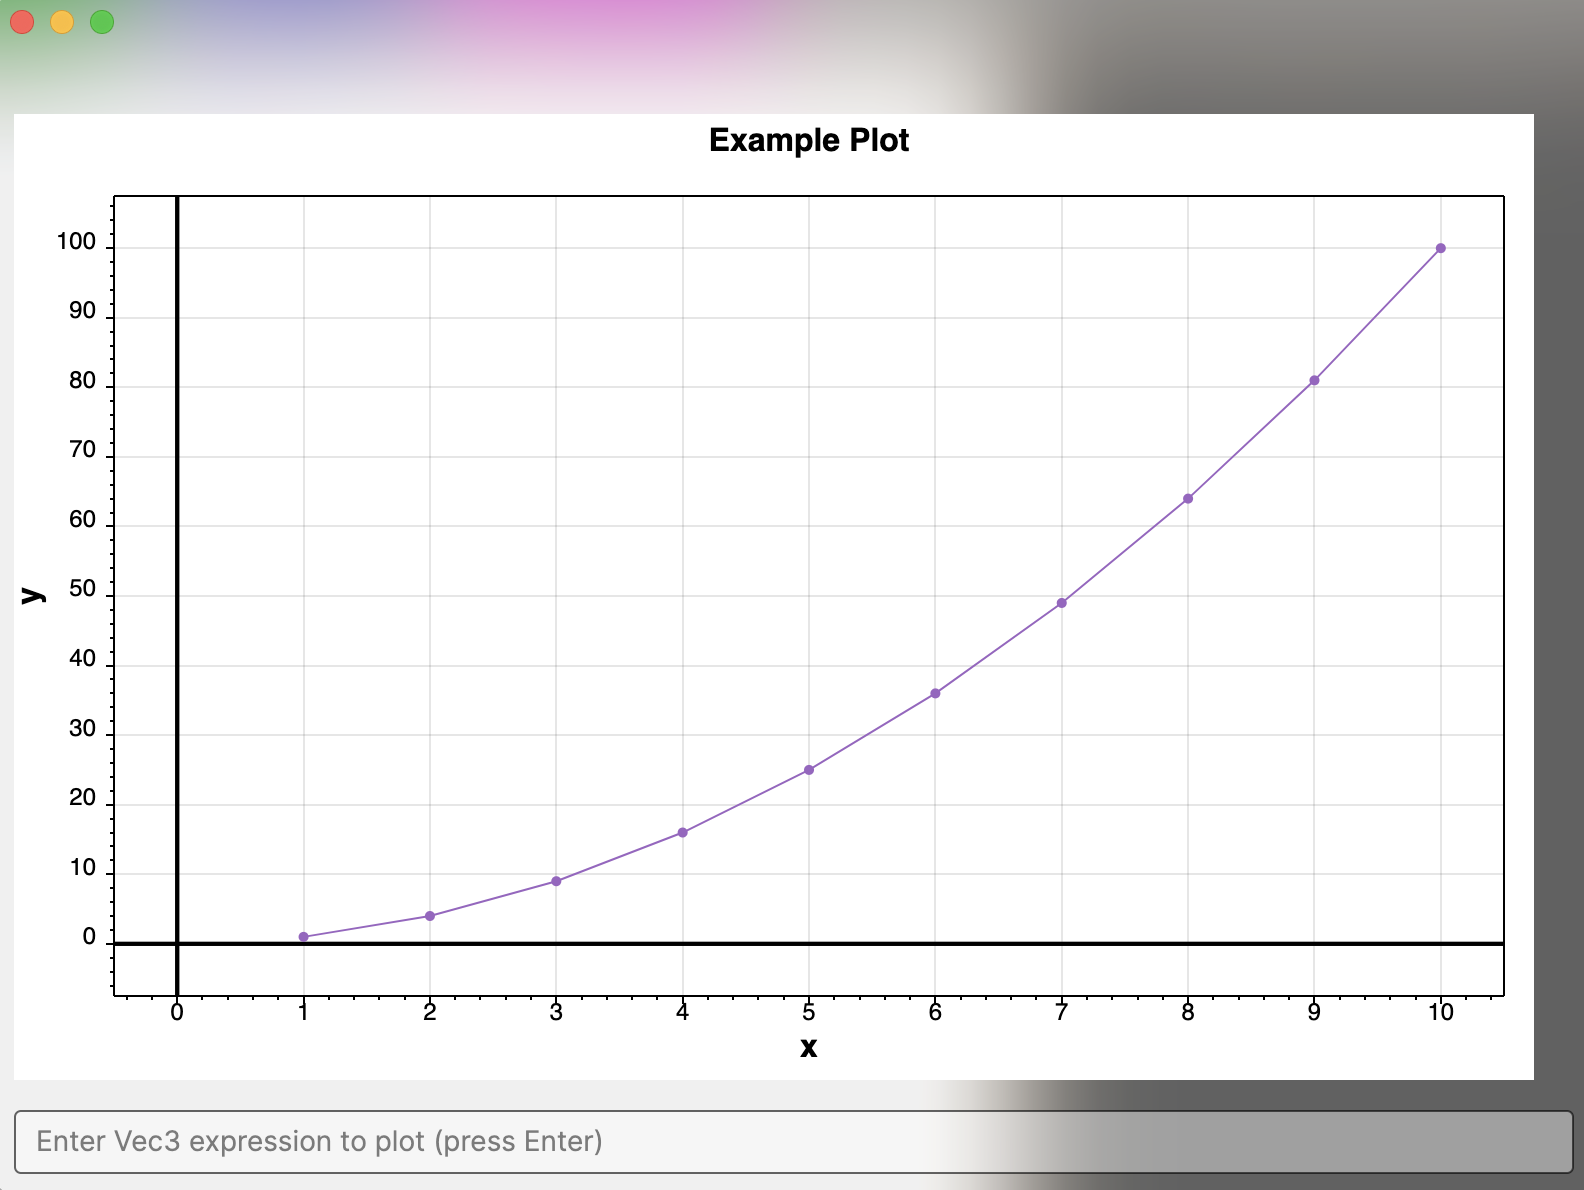
\includegraphics[width=0.8\textwidth]{assets/scatterPlot}
    \caption{Scatter plot}\label{fig:scatter-plot}
\end{figure}

The \textit{ptype} option allows for the user to specify the type of plot, with the options being \textit{bar},
\textit{scatter} and \textit{signal}.

The \textit{bar} type is useful for visualising data, the \textit{scatter} type is useful for plotting functions and
the \textit{signal} type is useful for plotting signals.
An example of a bar plot is shown in image~\ref{fig:bar-plot}.

\begin{figure}[H]
    \centering
    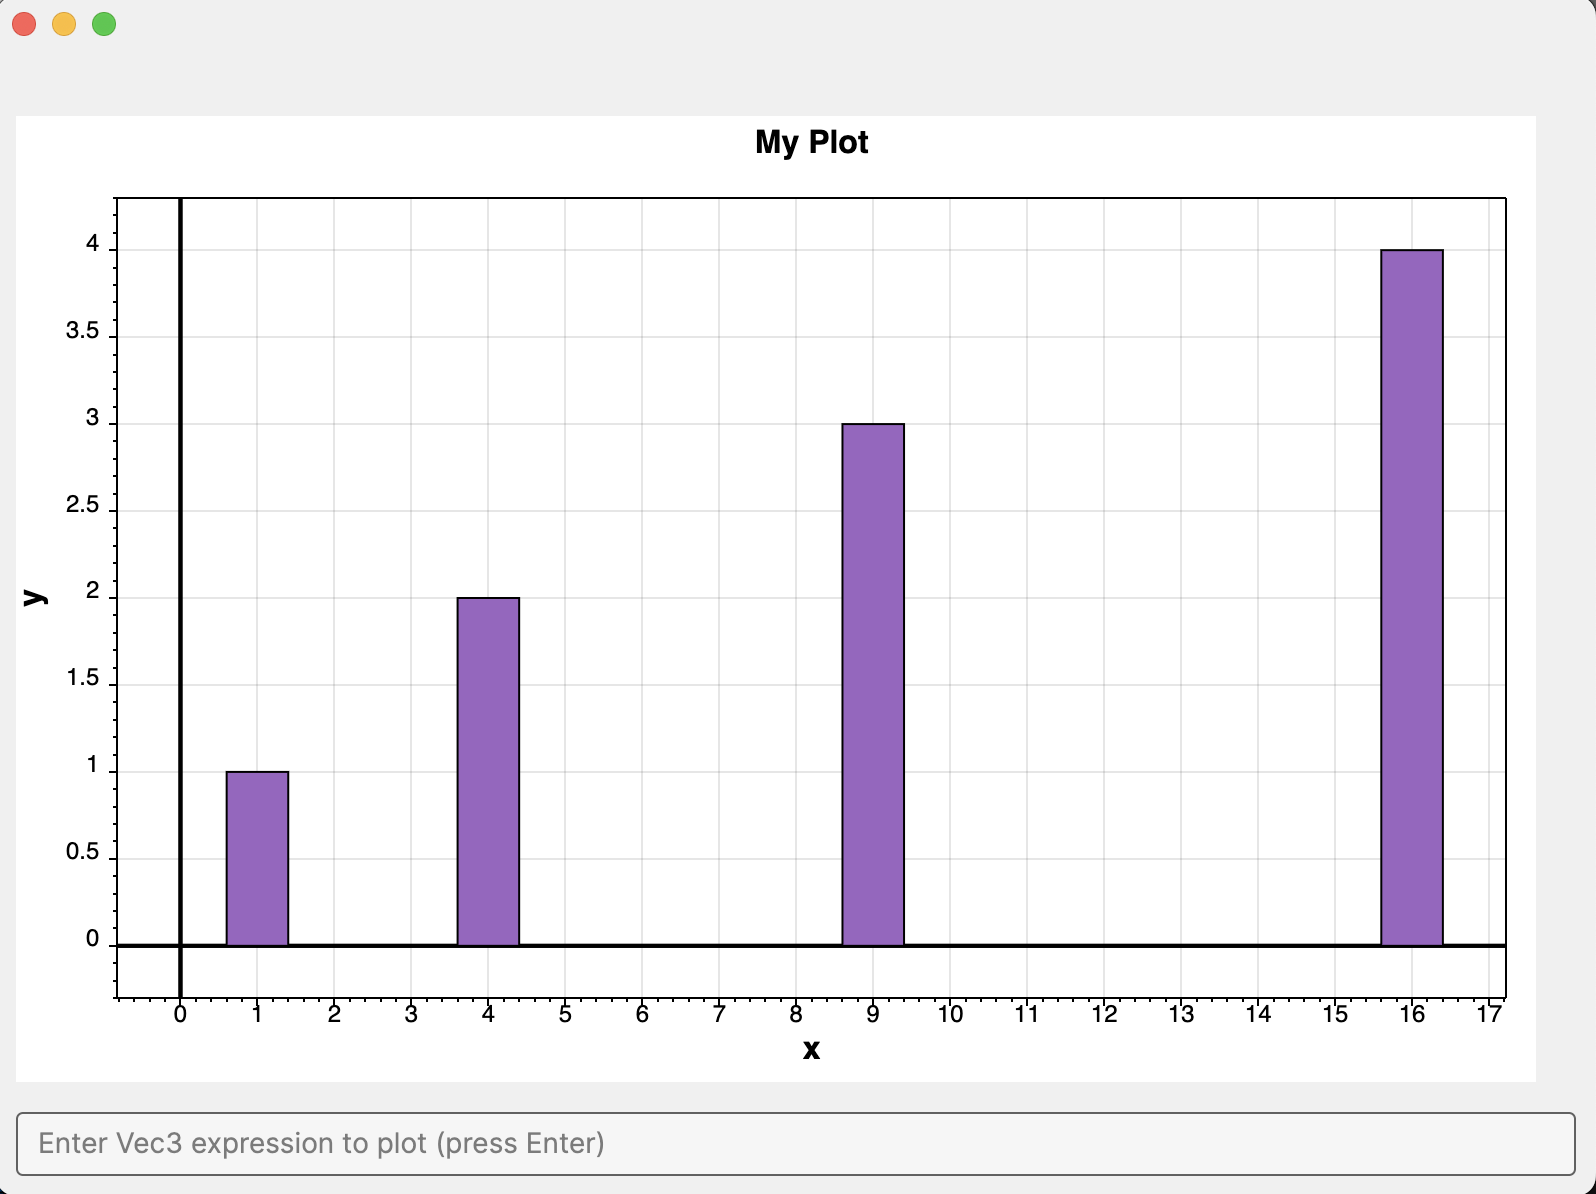
\includegraphics[width=0.8\textwidth]{assets/barChart}
    \caption{Bar plot}\label{fig:bar-plot}
\end{figure}

\paragraph{The \textit{plotFunc}} function takes in a string title and a pure function of type \textit{float -> float}.
The function is then plotted on the graph with an infinite range of x values.
Optionally, the user can also specify two more float values, \textit{start} and \textit{end}, in which case the 
integral of the function is calculated and displayed on the graph.

For example, given the following snippet:

\begin{minted}{fsharp}
let polynomial = (x) -> x^2 + 2.0 * x + 1.0
plotFunc("Polynomial", polynomial)
\end{minted}

Image~\ref{fig:polynomial-plot} shows the resulting plot.

\begin{figure}[H]
    \centering
    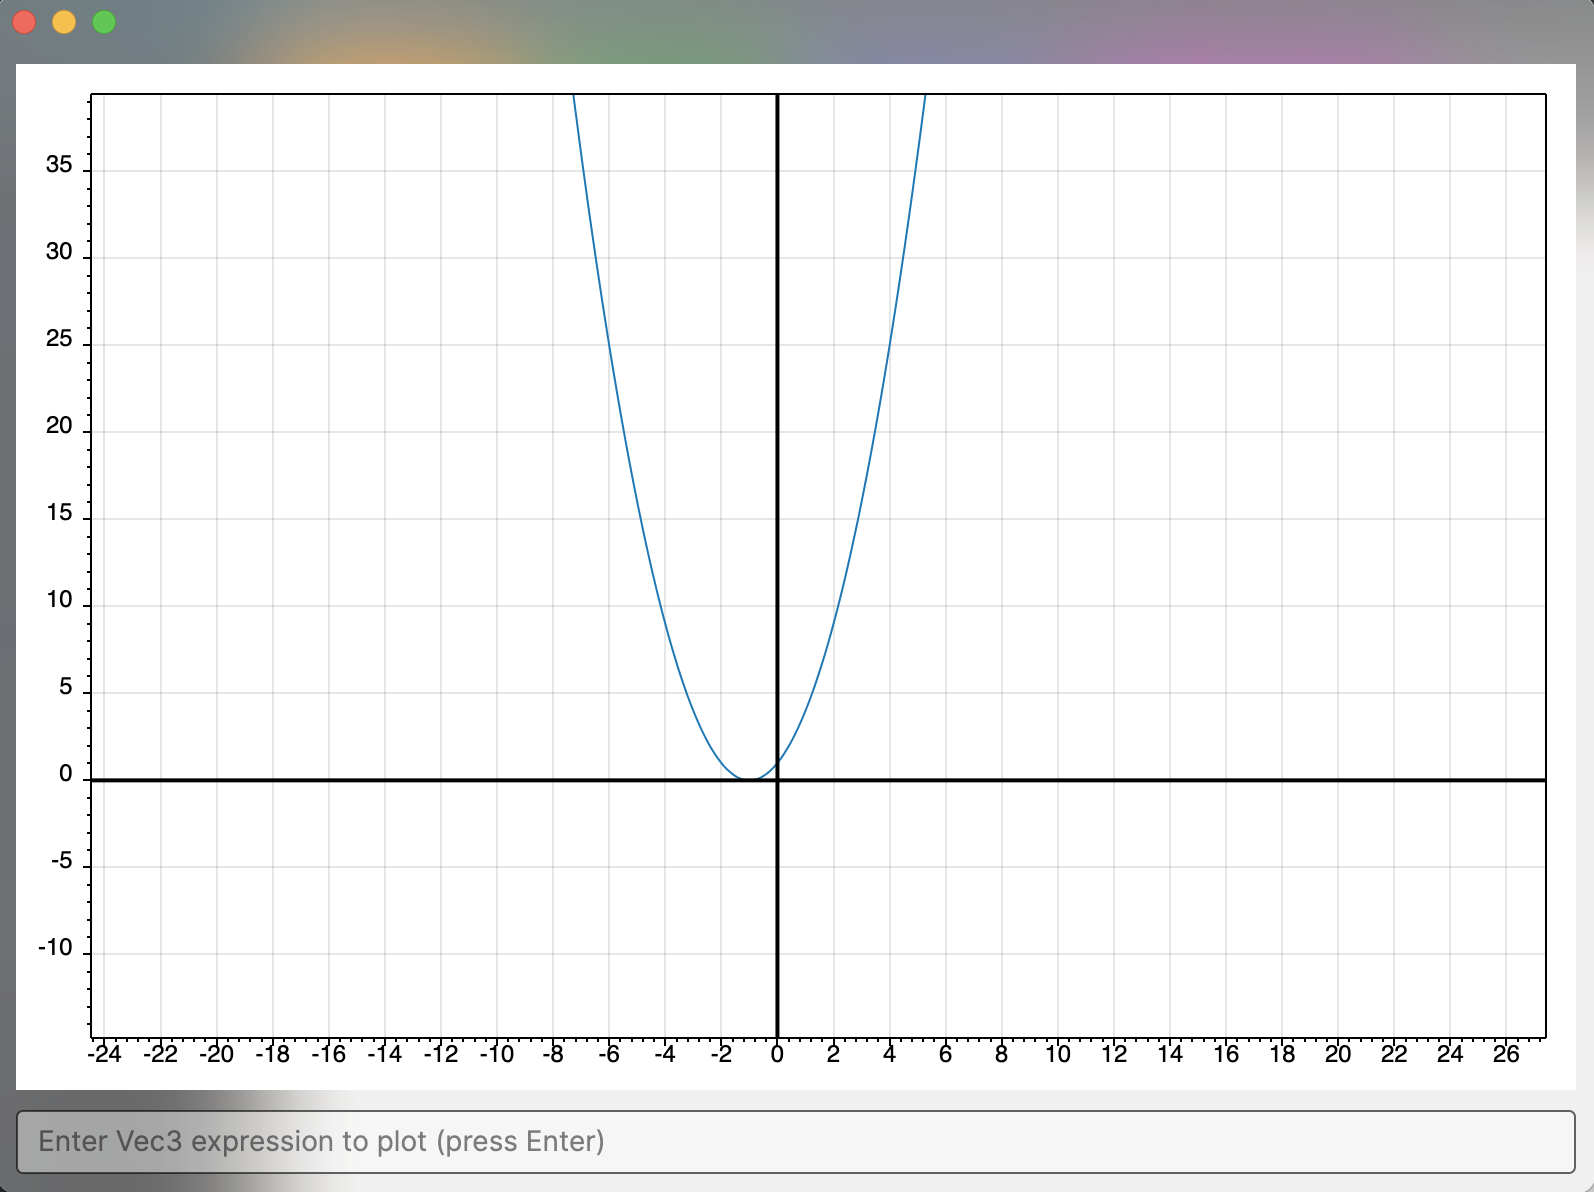
\includegraphics[width=0.8\textwidth]{assets/polynomialPlot}
    \caption{Polynomial plot}\label{fig:polynomial-plot}
\end{figure}

A point of interest is that for both the \textit{plotFunc} and \textit{plotFuncs} functions, a legend is provided 
with a textual representation of the function being plotted.
This is particularly useful when plotting multiple functions on the same graph, or when dynamically plotting 
functions (or their derivatives/integrals) based on user input.

\paragraph{The \textit{plotFuncs}} function takes in a string title and a list of pure functions of type 
\textit{$float \rightarrow float$}.
This allows for multiple plots to be placed on the same window, which we felt was valuable for comparing functions 
or plotting derivatives.
For example, given the following snippet:

\begin{minted}{fsharp}
let polynomial = (x) -> x^2 + 2.0 * x + 1.0
let derivate = differentiate(polynomial) // find the derivative of the polynomial
let integrand = integrate(polynomial) // find the integral of the polynomial
let tangentFunc = tangentFunc(polynomial, 2.0) // find the tangent function at x = 2.0

plotFuncs("Polynomial", [polynomial, derivate, integrand, tangentFunc])
\end{minted}

Image~\ref{fig:multiple-plots} shows the resulting plot.

\begin{figure}[H]
    \centering
    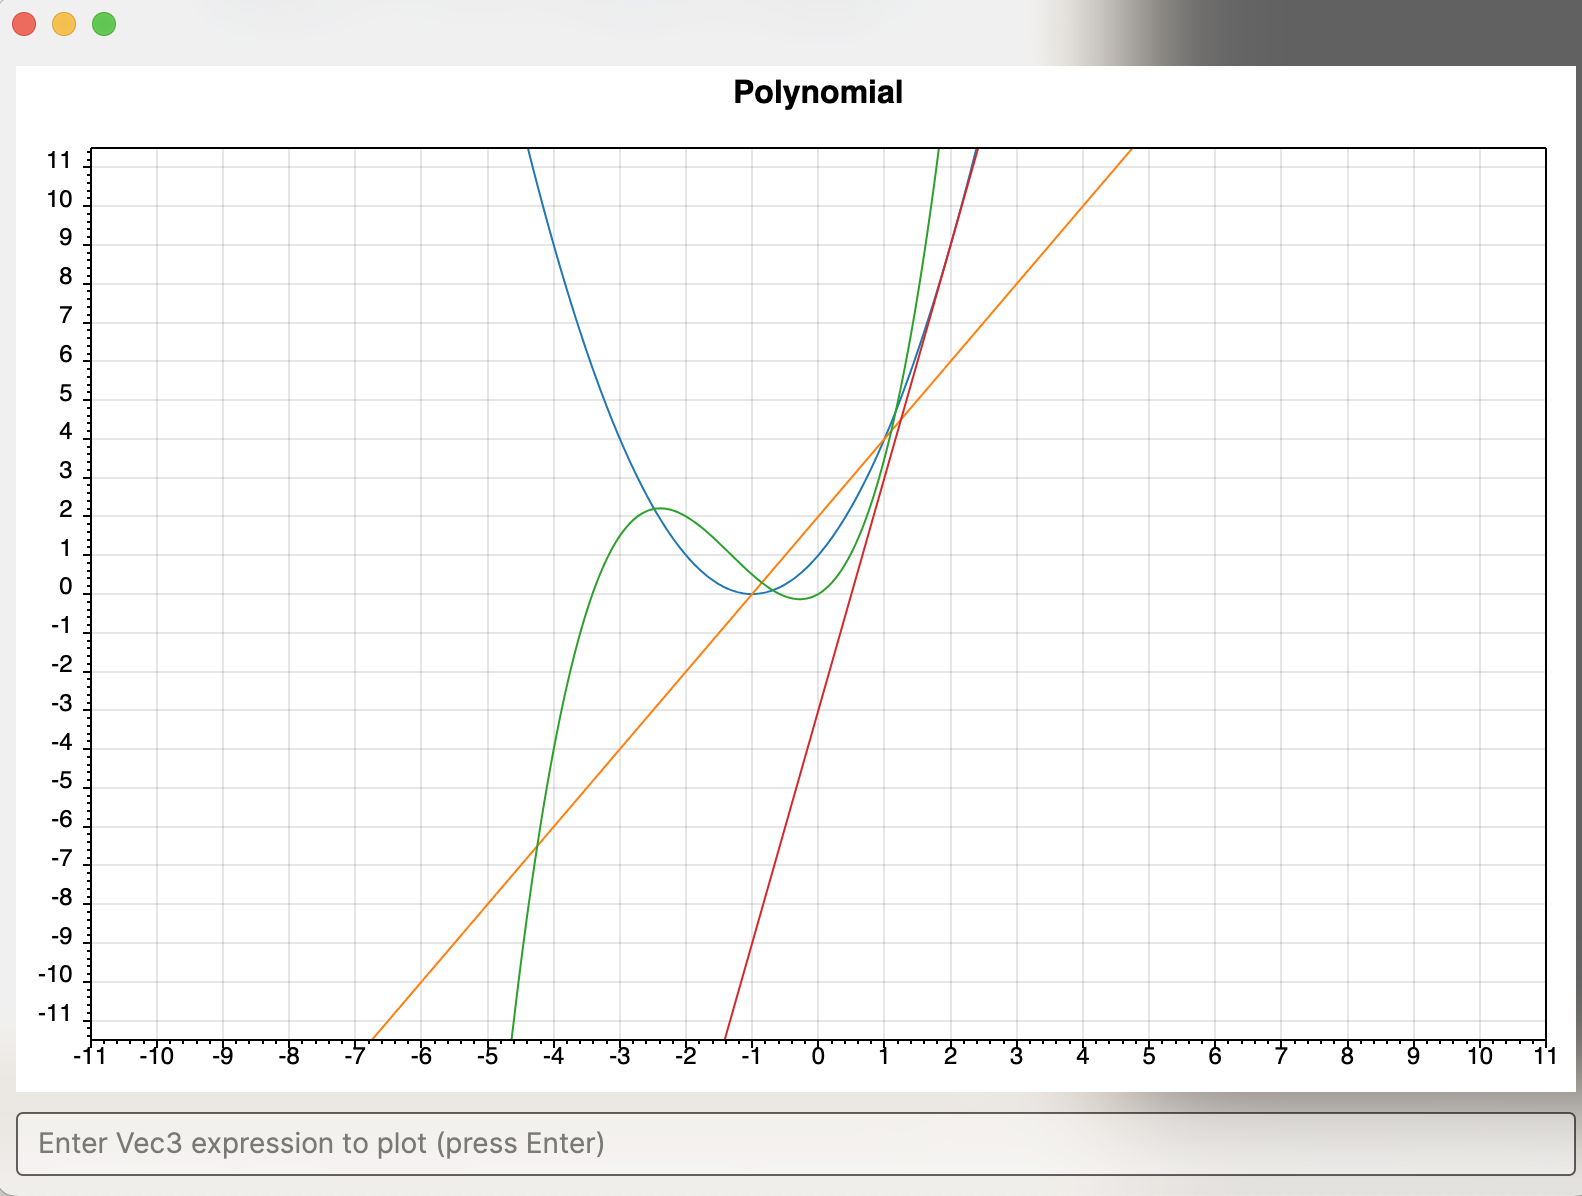
\includegraphics[width=0.8\textwidth]{assets/multiplePlots}
    \caption{Multiple plots}\label{fig:multiple-plots}
\end{figure}

The plots are very interactive, with the user being able to zoom in and out, move around and adjust the axes as
desired.

The plot windows also have an input at the bottom, which allows for the user to input a function and have it plotted
on command\ref{fig:plot-input}.
This is useful for quick visualisation of functions, and allows for a more interactive experience.
Note that variable resolution is performed on the input, allowing for the user to use variables defined in the
program in the input.
Additionally, the legend updates dynamically.

\begin{figure}[H]
    \centering
    
\includegraphics[width=0.8\textwidth]{assets/plotInput}
    
\includegraphics[width=0.8\textwidth]{assets/plotInput2}
    \caption{Plot input}\label{fig:plot-input}
\end{figure}

\section{Drawing}\label{sec:drawing}

As well as plotting, the user also has the option of drawing arbitrary shapes on a canvas, and attaching event 
listeners to them.
This is done by means of the \textit{draw} function, which takes in a record of configuration options of the following
type:

\begin{minted}{fsharp}
    type DrawConfig = {
        x: float,
        y: float,
        width: float,
        height: float,
        color: string,
        shape: "rectangle" | "circle",
        trace?: bool, 
    }
\end{minted}

Or a list of the above record type, allowing for multiple shapes to be drawn on the same canvas.

For example, the following will draw a few circles on the canvas:

\begin{minted}{fsharp}
let circle1 = {
    x = 100.0,
    y = 100.0,
    width = 50.0,
    height = 50.0,
    colour = "red",
    trace = true
}
let circle2 = {
    x = 200.0,
    y = 200.0,
    width = 50.0,
    height = 50.0,
    colour = "blue",
    trace = true
}
draw([circle1, circle2])
\end{minted}

The result of the above code is shown in image~\ref{fig:draw-circles}.

\begin{figure}[H]
    \centering
    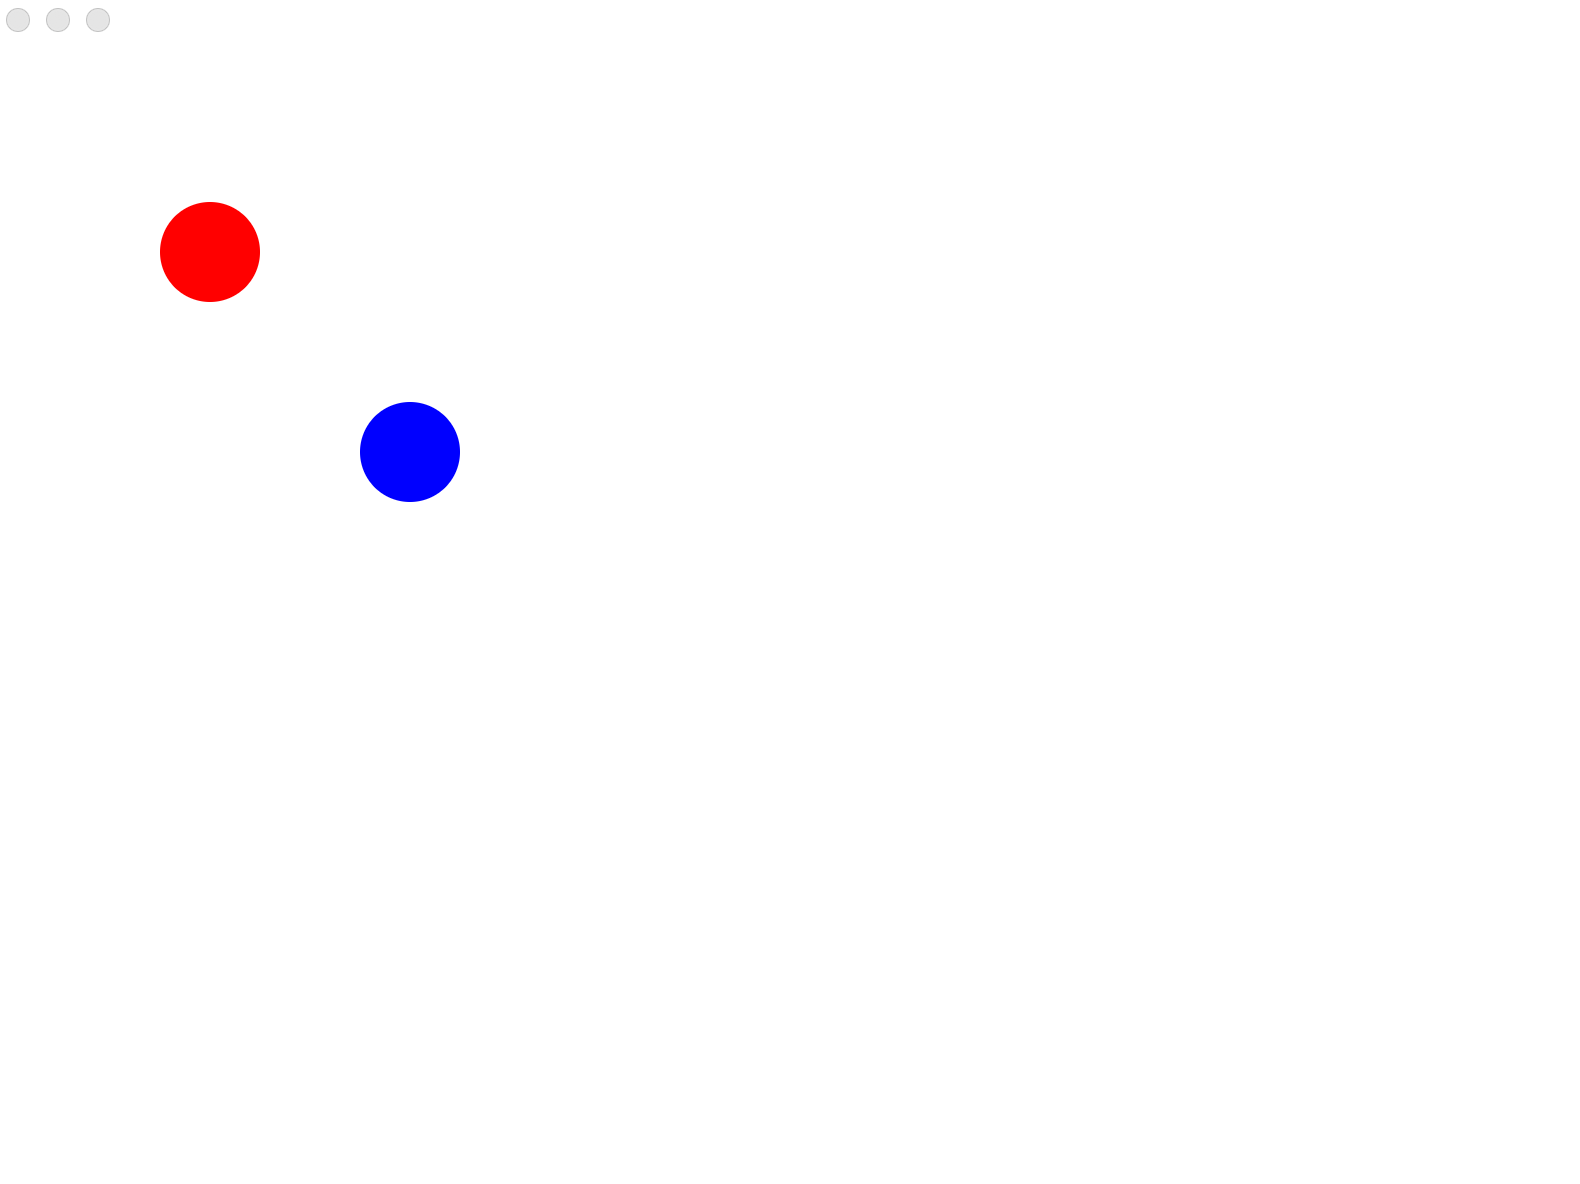
\includegraphics[width=0.8\textwidth]{assets/drawImage}
    \caption{Draw circles}\label{fig:draw-circles}
\end{figure}

The \textit{draw} function then returns a unique identifier for the shape, which can be used to attach event 
listeners, allowing for movement of the shape through key presses.

The following example attached event listeners to a shape which moves it left and right following the \textit{cos} curve:

\begin{minted}{fsharp}
on(id, Keys.Right, (state) -> { x = state.x + 10.0, y = cos(state.x) * 10.0 + 100.0 })
on(id, Keys.Left, (state) -> { x = state.x - 10.0, y = cos(state.x) * 10.0 + 100.0 })
\end{minted}

Where keys is a record defined in the prelude of the language (see~\autoref{sec:prelude}).

Additionally, the \textit{trace} option allows for the shape to leave a trail behind it, which can be useful for
animations or visualising movement.

\section{Transpiler Implementation} \label{sec:transpiler-implementation}
The Vec3 transpiler provides an alternative execution path by converting Vec3 programs into C code, enabling direct compilation to native machine code. This approach offers potential performance benefits while maintaining the language's semantics through careful mapping of Vec3's features to equivalent C constructs.
\subsection{Architecture Overview}
The transpiler follows a multi-phase pipeline that transforms Vec3 source code into executable programs. The process begins with the existing parser and type checker, then proceeds through code generation and compilation phases. Each phase is designed to be independent, allowing for easier maintenance and optimisation of individual components.
The transpilation process consists of the following main phases:
\begin{itemize}
\item Source code parsing and AST generation
\item Type checking and semantic analysis
\item C code generation
\item Compilation of generated C code to native executables
\end{itemize}
\subsection{Code Generation Strategy}
The code generator maps Vec3's high-level constructs to equivalent C implementations while preserving the language's semantics. 
This mapping is particularly careful in handling Vec3's functional features, which don't have direct equivalents in C. The generator maintains a reference counting system for memory management and implements a runtime environment that supports Vec3's dynamic features.
The transpiler generates C code that relies on a custom runtime library implementing Vec3's core features:
\begin{itemize}
\item Complex number arithmetic
\item First-class functions
\item Garbage collection through reference counting
\item Dynamic typing with runtime type checking
\item List and tuple operations
\item Record types with dynamic field access
\end{itemize}
\section{Memory Management and Garbage Collection}
\label{sec:memory-management}
The Vec3 runtime implements a deterministic memory management system through reference counting, offering predictable cleanup behavior while avoiding the complexity of tracing garbage collection. This approach particularly suits Vec3's transpiled nature, as it maps cleanly to C's manual memory management while providing automated cleanup semantics.
\subsection{Reference Counting Implementation}
The reference counting system centers around the Vec3Object structure, which serves as the base for all Vec3 values:
\begin{minted}{c}
typedef struct Vec3Object {
Type type;
int ref_count;
void (destructor)(struct Vec3Object);
} Vec3Object;
\end{minted}
Each object tracks its reference count, and the runtime provides two core operations:
\begin{minted}{c}
void vec3_incref(Vec3Value* value) {
if (value != NULL) {
value->object.ref_count++;
}
}
void vec3_decref(Vec3Value* value) {
if (value != NULL) {
assert(value->object.ref_count > 0);
value->object.ref_count--;
if (value->object.ref_count == 0) {
if (value->object.destructor) {
value->object.destructor((Vec3Object*)value);
}
free(value);
}
}
}
\end{minted}
\subsection{Destructor System}
The destructor function pointer in Vec3Object enables type-specific cleanup. Each value type can register its own destructor:
\begin{itemize}
\item Strings need to free their character buffer
\item Lists must decrement references to their elements
\item Functions must clean up their environment and name
\item Records must deallocate their hash table and decrement field references
\end{itemize}
This extensible destructor system ensures proper cleanup of complex data structures:
\begin{minted}{c}
void vec3_destroy_list(Vec3Object* object) {
Vec3Value* value = (Vec3Value*)object;
vec3_list* current = value->as.list;
while (current != NULL) {
vec3_list* next = current->next;
vec3_decref(current->value);
free(current);
current = next;
}
}
\end{minted}
\section{Generic Value Representation}
\label{sec:generic-value}
Vec3 implements a unified value representation that enables dynamic typing while maintaining efficiency. This design allows Vec3 to support multiple data types within a single value structure while providing type-safe operations.
\subsection{Value Structure}
The Vec3Value structure combines a type tag with a union of possible values:
\begin{minted}{c}
typedef struct {
Vec3Object object;
union {
Number number;
struct {
size_t length;
char* chars;
} string;
vec3_list* list;
bool boolean;
Vec3Function* function;
HashMap* record;
} as;
} Vec3Value;
\end{minted}
This design achieves several key objectives:
\begin{itemize}
\item Efficient memory usage through union-based storage
\item Fast type checking via the object type tag
\item Uniform handling of reference counting
\item Support for value-specific destructors
\end{itemize}
\subsection{Number System}
Vec3's number system demonstrates the flexibility of this approach by supporting multiple numeric types within a single representation:
\begin{minted}{c}
typedef struct {
NumberType type;
union {
int64_t integer;
double float_val;
struct { int64_t num; int64_t denom; } rational;
struct { double real; double imag; } complex;
} as;
} Number;
\end{minted}
This nested union structure allows Vec3 to efficiently represent different numeric types while maintaining type safety through the NumberType tag.
\subsection{Type-Safe Operations}
The value system includes comprehensive type checking and conversion operations. For example, the truthiness check demonstrates type-specific behavior:
\begin{minted}{c}
bool vec3_is_truthy(const Vec3Value* value) {
if (value == NULL || value->object.type == TYPE_NIL) {
return false;
}
\subsection{Function Translation}
One of the more complex aspects of the transpiler is the translation of Vec3's first-class functions to C. The transpiler generates wrapper structures that capture the function's environment and parameters:
\begin{minted}{c}
typedef struct {
char* name;
int arity;
Vec3Value* (fn)(Vec3Value* args);
struct Vec3Env* env;
bool is_recursive;
} Vec3Function;
\end{minted}
This structure enables proper handling of closures and maintains Vec3's lexical scoping rules in the generated C code. 
The transpiler pays special attention to recursive functions, implementing them through a trampolining mechanism to prevent stack overflow in tail-recursive cases.
\section{Plotting}\label{sec:plotting}

The plotting system in Vec3 is built on top of GnuPlot, providing a powerful and flexible interface for data visualization. GnuPlot was chosen for its robust plotting capabilities, wide range of plot types, and ability to generate high-quality visualizations. The system interfaces with GnuPlot through pipes, allowing for real-time updates and interactive manipulation of plots.

\subsection{Core Plotting Functions}\label{subsec:core-plotting-functions}

The language provides three main plotting functions: \textit{plot}, \textit{plotFunc}, and \textit{plotFuncs}. Each serves a distinct purpose in data visualization:

\textit{plot} takes a configuration record containing the plot title, type, and data series. It supports various plot types including scatter plots, line plots, bar charts, and signal plots. The configuration is passed as a list of key-value pairs:

\begin{minted}{fsharp}
plot([
    "title" -> "Plot Title",
    "ptype" -> "scatter",  // or "line", "bar", "signal"
    "x" -> [x_values],
    "y" -> [y_values]
])
\end{minted}

\textit{plotFunc} specializes in visualizing mathematical functions. It takes a title string and a function that maps real numbers to real numbers, plotting the function over the domain [-10, 10]:

\begin{minted}{fsharp}
plotFunc("Title", f)  // where f: float -> float
\end{minted}

\textit{plotFuncs} extends this capability to multiple functions, allowing for comparative visualization. Functions are plotted in different colors with an automatically generated legend:

\begin{minted}{fsharp}
plotFuncs("Title", [f1, f2, ...])
\end{minted}

\begin{figure}[H]
    \centering
    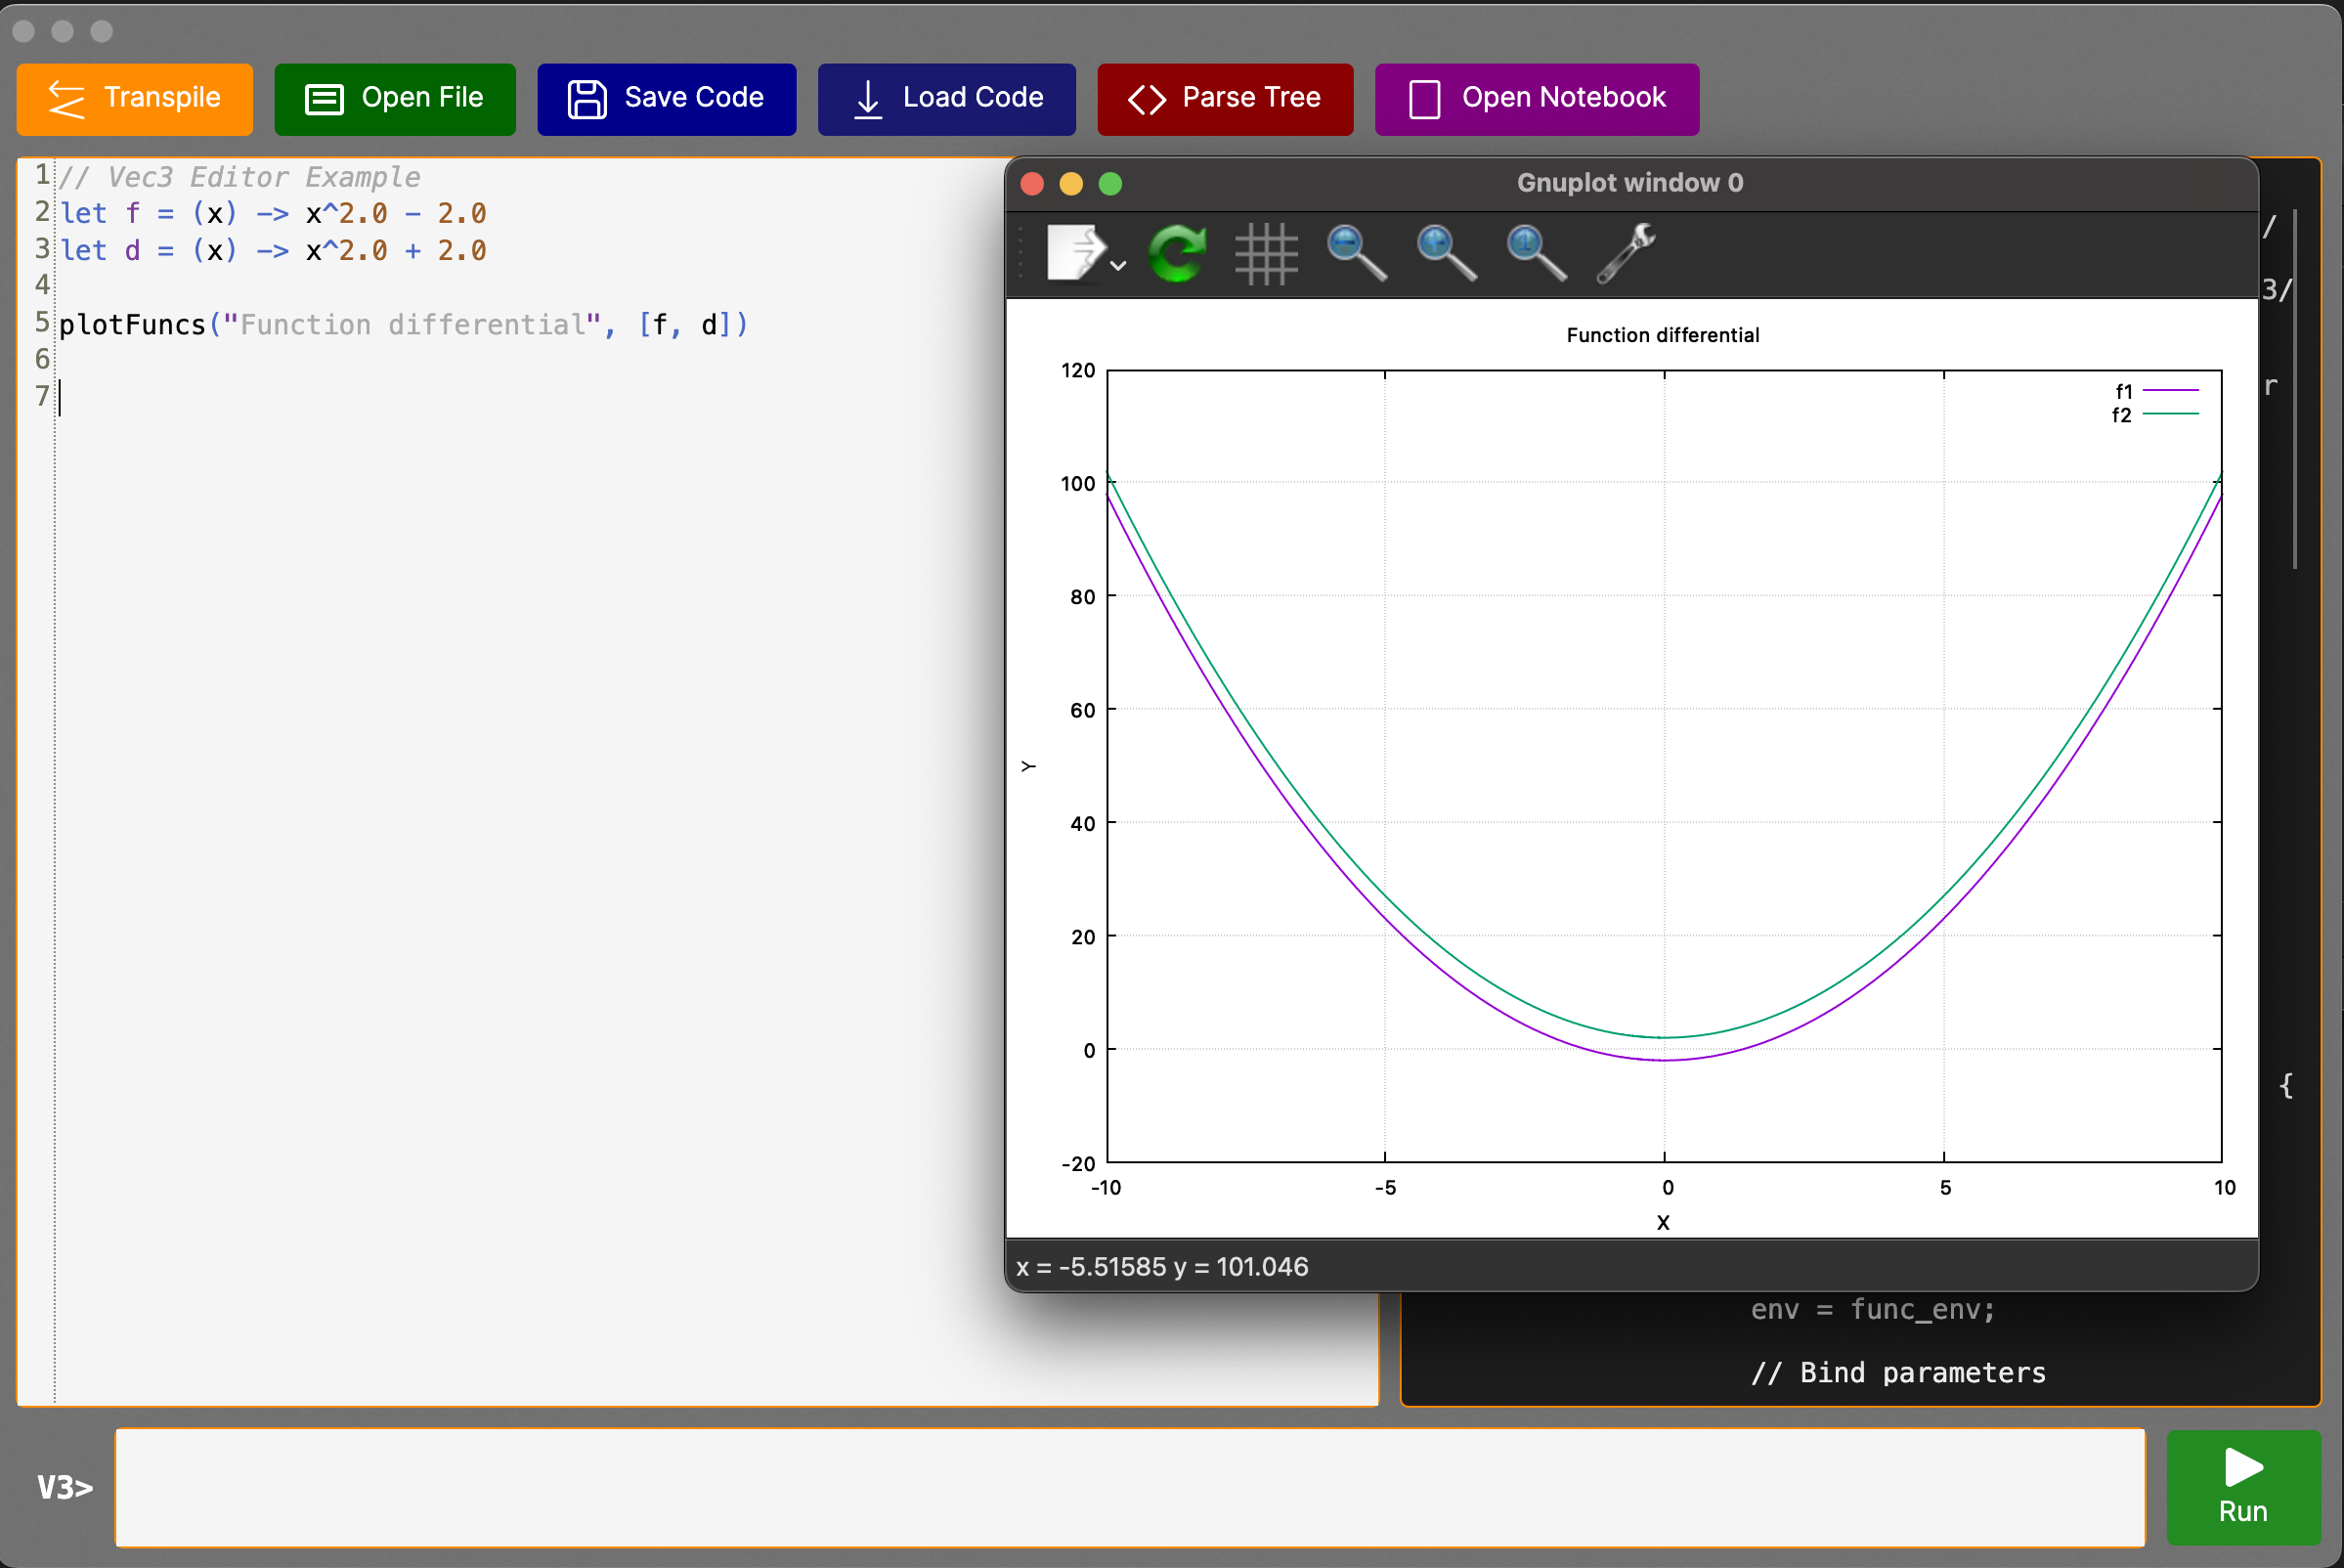
\includegraphics[width=0.8\textwidth]{assets/gnuplot.png}
    \caption{Example GnuPlot output showing two parabolas}\label{fig:gnuplot-example}
\end{figure}

Figure~\ref{fig:gnuplot-example} demonstrates the output of \textit{plotFuncs} with two parabolic functions:

\begin{minted}{fsharp}
let f = (x) -> x^2.0 - 2.0     // Upward parabola shifted down
let d = (x) -> -x^2.0 + 2.0    // Downward parabola shifted up
plotFuncs("Function differential", [f, d])
\end{minted}

The purple line shows $f(x) = x^2 - 2$, while the green line shows $d(x) = -x^2 + 2$. This example demonstrates the system's ability to handle multiple functions and generate clear, distinguishable plots.

\subsection{Implementation Details}\label{subsec:plotting-implementation}

The plotting system communicates with GnuPlot through pipes, sending commands and data for real-time plot generation. The implementation handles memory management, data conversion, and proper cleanup of GnuPlot processes. Error handling ensures robust operation, with clear error messages for common issues like invalid function inputs or plotting errors.

GnuPlot's native features are exposed through the Vec3 interface, including:
\begin{itemize}
    \item Interactive zooming and panning
    \item Configurable plot styles and colors
    \item Automatic axis scaling
    \item Grid lines and legends
    \item Multiple plot types
\end{itemize}
The system automatically handles data conversion between Vec3's number types and GnuPlot's expected formats, ensuring accurate plotting regardless of the input number type (integer, float, rational, or complex).

\subsection{Error Handling}
The transpiler implements comprehensive error handling throughout the generation process. 
It categorises errors into these distinct types:
\begin{itemize}
\item IOError for file system and input/output operations
\item ParseError for syntax and parsing failures
\item TypeError for type checking violations
\item CodeGenError for code generation issues
\item CompilationError for C compiler errors
\end{itemize}
This granular error categorisation helps developers quickly identify and fix issues in their Vec3 programs, whether they occur during parsing, type checking, code generation, or final compilation.
\subsection{Build System Integration}
The transpiler includes a configurable build system that manages the compilation pipeline. It handles directory structure creation, runtime library inclusion, and compiler invocation. The system is designed to be platform-independent, automatically adjusting paths and compiler commands based on the operating system:
\begin{minted}{fsharp}
type TranspilerConfig =
{ OutputDir: string
RuntimeDir: string
IncludeDir: string
CompilerPath: string }
\end{minted}
This configuration system ensures consistent behavior across different development environments while maintaining flexibility for different deployment scenarios.

\subsection{Performance Considerations}
The transpiler's output prioritises runtime performance through several optimisation strategies:

\begin{itemize}
\item Minimises dynamic memory allocations where possible
\item Implements efficient reference counting mechanisms
\item Generates code that can benefit from the C compiler's optimisations
\item Structures code to enable the C compiler's full range of optimisations
\item Produces code patterns that potentially outperform interpreted execution
\end{itemize}

\section{Future Developments}
While the current transpiler implementation successfully handles the core Vec3 language features, several areas present opportunities for future enhancement:
\begin{itemize}
\item Optimisation of generated code patterns
\item Improved debug information generation
\item Integration with profile-guided optimisation techniques
\item Enhanced cross-platform compatibility
\item Expanded runtime library capabilities
\end{itemize}

The modular design of the transpiler makes it well-suited for such future expansions while maintaining its current reliability and functionality.

\section{Code architecture}\label{sec:code-architecture}
The solution is split into 3 separate projects: the GUI, Tests and the main interpreter / compiler project.
\paragraph{The GUI} is where the project runs from, and is a standard Avalonia project, with a main window (the code editor), 
and then some other windows for the plots, drawing and notebook view, as well as some non-UI files such as the a helper 
module for PDF exports.
It also contains a directory containing the prelude and standard library of the language, which are then imported as 
desired (except the prelude, which is always implicitly imported).
The frameworks are libraries used in the GUI project include AvaloniaUI, AvaloniaEdit, FSharp.Core, ScottPlot, 
TextMate and QuestPDF\@. 
\paragraph{The Tests} project mirrors the main project, with a similar structure and file naming for clear and sensible
organisation.
It uses the NUnit framework for testing, and tests the lexer, parser, compiler and type inference.
\paragraph{The main project} is where the main interpreter and compiler are implemented, and is split into the following
submodules:
\begin{itemize}
    \item \textit{Syntax Analysis} contains the lexer and parser, as well as the AST of the language.
    \item \textit{Type Analysis} contains the type inference engine.
    \item \textit{Backend} contains the compiler and virtual machine.
    \item \textit{Optimisation} contains the optimisation passes (dead code elimination and constant folding).
\end{itemize}
A couple more files, such as the REPL, which contains helper functions for compilation and running of code, and the
Symbolic Expression modules, which contain helper functions for maths operations such as simplification of formulas 
and calculation of derivatives, are also present.
No external libraries are used in the main project, as it is a standalone F\# project.

We felt this structure was sensible, as it allowed for clear separation of concerns and easy navigation of the codebase.

